\documentclass[11pt]{article}

\usepackage[margin=1.1in]{geometry}
\usepackage{graphicx}
\usepackage{amsmath}
\usepackage{amssymb}
\usepackage{booktabs}
\usepackage{makecell}
\providecommand{\cmark}{\checkmark}
\providecommand{\xmark}{\ensuremath{\times}}
\usepackage[authoryear,round]{natbib}
\usepackage{microtype}
\usepackage{etoolbox}
\usepackage{hyperref}
\hypersetup{colorlinks=true, linkcolor=blue, citecolor=blue, urlcolor=blue}

% --- JSS-style compatibility macros (frontmatter written for jss.cls) -------
\newcommand{\pkg}[1]{\textbf{#1}}
\newcommand{\proglang}[1]{\textsf{#1}}
\providecommand{\code}[1]{\texttt{#1}}
\newcommand{\Plainauthor}[1]{}
\newcommand{\Plaintitle}[1]{}
\newcommand{\Plainkeywords}[1]{}
\newcommand{\Keywords}[1]{\par\medskip\noindent\textit{Keywords:} #1\par\medskip}
\renewcommand{\And}{\and}
\providecommand{\AND}{\and}
\renewcommand{\AND}{\and}

% The frontmatter file sets \title/\author/\date and then opens the abstract;
% emit the title block just before the abstract begins.
\BeforeBeginEnvironment{abstract}{\maketitle}

\begin{document}

\title{\pkg{amore}: A Unified Case-Control Partial-Likelihood Toolchain for
Simulating, Fitting, and Checking Relational and Hyper-Event Models in \proglang{R}}

\author{
  Francisco Richter \\ Universit\`a della Svizzera italiana
  \And
  Martina Boschi \\ Universit\`a della Svizzera italiana
  \AND
  Melania Lembo \\ Universit\`a della Svizzera italiana
  \And
  Ernst C. Wit \\ Universit\`a della Svizzera italiana
}

\Plainauthor{Francisco Richter, Martina Boschi, Melania Lembo, Ernst C. Wit}
\Plaintitle{amore: A Unified Case-Control Partial-Likelihood Toolchain for
Simulating, Fitting, and Checking Relational and Hyper-Event Models in R}

\date{}

\begin{abstract}
Relational event models describe how interactions in a network unfold in
continuous time, with intensities driven by the history of past events.
Recent methodological advances --- timing and closure variants of the
endogenous statistics, smooth and time-varying effects, global covariates,
hyper-events, and martingale-residual goodness-of-fit tests --- have so far
lived in separate implementations, making complete analyses difficult to
carry out and to reproduce. We present \pkg{amore}, an \proglang{R} package
that brings the full workflow --- simulation, case-control sampling,
endogenous-statistic construction, estimation, and model checking --- under
a single case-control partial likelihood. The estimation framework offers a
spectrum of intensity specifications behind one interface: a linear
conditional logit, smooth additive effects --- fitted in memory or, at scale,
by stochastic gradient over per-covariate spline bases --- and a neural
network scoring the full covariate vector, trading interpretability against
flexibility in a controlled way. A generative engine simulates from the
same model class it estimates, which yields an internal consistency check:
statistics computed during simulation and reconstructed from the event
history agree to numerical precision, and effects planted in simulation are
recovered in estimation. We illustrate the workflow on classroom,
e-mail, and social-network event data.
\end{abstract}

\Keywords{relational event models, partial likelihood, case-control sampling,
network event data, goodness of fit, \proglang{R}}
\Plainkeywords{relational event models, partial likelihood, case-control
sampling, network event data, goodness of fit, R}


\section{Introduction}
\label{sec:introduction}

Relational event models (REMs) describe streams of time-stamped, directed
interactions --- emails between colleagues, messages in a classroom, citations
between documents, trips in a bike-sharing network --- as the realisations of a
continuous-time point process whose instantaneous rate depends on the history of
the network itself \citep{butts2008, bianchi2024}. A recent line of methodological work has extended this framework rapidly: timing,
closure and actor-heterogeneity effects \citep{juozaitiene2024}, models with
global covariates and a time-shift non-event sampling scheme
\citep{lembo2025}, martingale-residual goodness-of-fit diagnostics
\citep{boschi2025gof}, and relational \emph{hyper}-event models (RHEMs) with
time-varying non-linear effects \citep{boschi2025rhem, lerner2023}. Each
contribution is statistically self-contained and well-validated, but the
software that accompanies them is not: the methodology currently lives as
bespoke analysis scripts accompanying the individual papers, supplemented by
the Java tool \pkg{eventnet} for hyper-event feature extraction \citep{lerner2023}.
A practitioner who wants to simulate a network, sample non-events, compute
endogenous statistics, fit a model, and check its fit must today assemble these
stages by hand from heterogeneous sources.

The CRAN-native alternative does not close this gap either. The Tilburg
network group ships a mature, modular stack --- \pkg{remify}, \pkg{remstats},
\pkg{remstimate} for the analysis pipeline and \pkg{remulate} for simulation
\citep{lakdawala2025} --- but it is confined to \emph{linear} effects on the
log-rate and splits simulation from inference across separate packages with
distinct data contracts. The smooth, time-varying, and non-linear effects that
motivate much of this recent work, and the goodness-of-fit machinery
that accompanies them, have no home in that ecosystem. There is, in short, no
single tested R package that carries a relational (or hyper-relational) event
analysis from a simulated or observed event log all the way through to a fitted
model and its diagnostics.

\begin{table}[ht]
\centering\small
\begin{tabular}{lcccc}
\toprule
Capability & \pkg{amore} & \pkg{relevent} & \makecell{\pkg{remstats}\\stack$^{\dagger}$} & \makecell{\pkg{eventnet}\\(Java)} \\
\midrule
Linear endogenous effects        & \cmark & \cmark & \cmark & $\circ$ \\
Smooth / non-linear / time-varying & \cmark & \xmark & \xmark & \xmark \\
Random effects / frailty          & \cmark & $\circ$ & \xmark & \xmark \\
Flexible effects at scale (neural / SGD) & \cmark & \xmark & \xmark & \xmark \\
Event simulation                  & \cmark & \cmark & $\circ$ & \xmark \\
Case-control non-event sampling   & \cmark & \xmark & $\circ$ & \cmark \\
Residual-based goodness of fit    & \cmark & \xmark & \xmark & \xmark \\
Hyper-event (set-valued) support  & \cmark & \xmark & \xmark & \cmark \\
Single package, one data contract & \cmark & $\circ$ & \xmark & \xmark \\
\bottomrule
\end{tabular}
\caption{Primary documented scope of relational-event software, relative to
\pkg{amore}. \cmark: supported in the package; $\circ$: supported in
restricted form, in a companion package, or as an external tool; \xmark:
absent. The comparison reflects the packages' documented capabilities as of
the cited versions and is necessarily coarse. $^{\dagger}$The Tilburg stack
(\pkg{remify}, \pkg{remstats}, \pkg{remstimate}, \pkg{remulate};
\citealp{lakdawala2025}) is modular: simulation (\pkg{remulate}) and inference
are separate packages with distinct data contracts, and the estimation
pipeline is restricted to linear effects on the log-rate.
\pkg{eventnet} \citep{lerner2023} is a Java feature-extraction tool, including
hyper-event statistics and nested case-control sampling, paired with external
model fitting. \pkg{relevent} \citep{butts2008} is the original \proglang{R}
REM implementation, covering linear models and simulation.}
\label{tab:landscape}
\end{table}

Table~\ref{tab:landscape} situates \pkg{amore} against the main alternatives.
No existing tool offers smooth, neural, and goodness-of-fit machinery within a
single simulation-to-diagnostics workflow; that combination, rather than any
individual capability, is what \pkg{amore} contributes.

\subsection{What \pkg{amore} provides}
\label{sec:what-amore-provides}

\pkg{amore} closes that loop: a single \proglang{R} package in which this
strand of relational event methodology becomes one coherent workflow
spanning five stages:

\begin{enumerate}
  \item \emph{simulation} of event streams by an exact Gillespie algorithm or an
  approximate tau-leap scheme sharing one endogenous-state machine
  (\code{simulate\_relational\_events});
  \item \emph{case-control non-event sampling}, including the \citet{lembo2025}
  time-shift scheme for global covariates, with sampling scopes for repeatable
  and non-repeatable processes (\code{sample\_non\_events});
  \item a history-aware \emph{endogenous-statistics engine} covering the
  full catalogue of timing and closure variants
  (\code{compute\_endogenous\_features});
  \item a single \emph{model-fitting} front-end, \code{rem()}; and
  \item the \citet{boschi2025gof} \emph{martingale-residual goodness-of-fit}
  family for the linear case-control fit (\code{gof\_univariate},
  \code{gof\_multivariate}, \code{gof\_global}, \code{gof\_auxiliary}).
\end{enumerate}

The five stages share one data contract --- the \code{amore\_event\_log} ---
so that the output of the simulator feeds the sampler, whose output feeds the
feature engine, whose output feeds \code{rem()} directly. Correctness across
the seam between simulation and post-hoc analysis is enforced by a
cross-implementation parity oracle (the simulator's
on-the-fly statistics are compared against the independently coded post-hoc
engine to a tolerance of $4.3\times10^{-14}$ under aligned histories), backed
by an extensive automated test suite.

\subsection{One likelihood, a spectrum of predictors}
\label{sec:one-likelihood}

The expository spine of the package is a single estimand viewed through three
fitting backends, selected by \code{rem(method = c("gam", "clogit", "nn"))}.
Two of these maximise \emph{the same} objective: the risk-set softmax
conditional-logistic partial likelihood that arises when the continuous-time
REM intensity is reduced, via case-control sampling, to a conditional
multinomial choice among the realised event and its sampled non-events
\citep{lerner2020}. The \code{clogit} backend fits this partial likelihood with
a linear predictor through \pkg{survival}; the \code{nn} backend maximises the
identical per-stratum objective with a multilayer-perceptron predictor and
hand-derived analytic gradients. The third backend, \code{gam}, fits the
\emph{algebraically related} degenerate case-1-control binomial logistic
regression of \citet{boschi2025gof, juozaitiene2024} through \pkg{mgcv}, which
unlocks smooth, time-varying, non-linear, and random-effect terms. We are
deliberately precise about this distinction: the \code{gam} backend is not a
risk-set softmax fit and coincides with a two-element conditional logit only
under a single matched control, a condition \code{rem()} does not enforce.
What \code{rem()} offers is therefore not one likelihood maximised three ways,
but a single front-end and a shared \code{rem} S3 contract spanning a
spectrum of predictors --- linear, smooth, and neural --- over closely related
case-control objectives. To our knowledge no prior work presents this
linear-to-smooth-to-neural progression as one workflow behind one interface.

\subsection{What this paper does not claim}
\label{sec:scope}

Because \pkg{amore} sits squarely inside an active methodological literature,
we state its boundaries plainly. \emph{The contribution is software and
synthesis, not new statistics.} Every estimator, sampling scheme, and
diagnostic implemented here is published or derives directly from the
published literature; \pkg{amore}'s value is the integrated, documented, tested, and
reproducible artifact, together with the unifying frame of
Section~\ref{sec:one-likelihood}.

In particular, the \code{nn} backend is \emph{not} a claim to the first neural
REM. Flexible-effect relational event modelling at scale already exists:
STREAM \citep{filippimazzola2024} fits additive B-spline effects by minibatch
stochastic gradient descent on the same nested case-control objective, scaling
to $10^{8}$ patent citations, and the neural temporal-point-process literature
--- recurrent marked temporal point processes \citep{du2016}, the neural
Hawkes process \citep{mei2017}, dynamic-graph representation learning
\citep{trivedi2019}, and the review by \citet{shchur2021} --- long predates
this package. What
\pkg{amore}'s \code{nn} backend contributes is accessibility and engineering: a
GPU-free, zero-extra-dependency, pure-R neural conditional-logit backend,
reachable by \code{install.packages()}, whose analytic gradients are
verified against numerical differentiation (agreement to
$1.4\times10^{-10}$), and which --- by scoring the full candidate vector
jointly rather than additively --- can learn cross-feature interactions and
recover them post-hoc through partial-dependence plots. Its reported
concordance figures are \emph{in-sample}; it provides no uncertainty
quantification (\code{coef()} returns \code{NULL}, there are no standard errors
or variance-covariance estimates), it trains by gradient descent in pure R
(full-batch by default, with optional mini-batching), and it does not accept
factor covariates. We make no scalability or inferential claim
for it. Finally, the goodness-of-fit family is restricted to the linear
case-control fit (\code{rem()} rejects non-linear specifications before any GOF
computation), and the RHEM hyper-event statistics, while \code{rem}-ready, are
not yet demonstrated end-to-end on a fitted hyper-event model.

\subsection{Contributions}
\label{sec:contributions}

We organise the contribution in three tiers, from the core deliverable to
supporting material.

\paragraph{Primary: software and synthesis.}
\pkg{amore} is, to our knowledge, the first \proglang{R} package that closes
the full REM/RHEM loop --- simulate, sample non-events, compute features,
fit, and check --- for these recent formulations
\citep{juozaitiene2024, lembo2025, boschi2025gof, boschi2025rhem}, which
have so far been available only as scattered analysis scripts and the Java
\pkg{eventnet} tool, while existing CRAN packages cover linear effects and
split simulation from inference. The accompanying expository frame --- one
front-end and one S3 contract over a linear-to-smooth-to-neural spectrum of
predictors built on closely related case-control objectives
(Section~\ref{sec:one-likelihood}) --- is, as far as we are aware, not
articulated as a single workflow elsewhere.

\paragraph{Software contributions.}
The package ships with strong validation evidence, including a genuine
cross-implementation oracle: simulator-versus-post-hoc feature parity to
$4.3\times10^{-14}$ under aligned histories, planted-effect recovery under both
simulation schemes, an analytic-versus-numerical gradient check for the neural
backend ($1.4\times10^{-10}$), and the goodness-of-fit identities (including an
analytic single-component reduction verified to $10^{-10}$). The
pure-R neural conditional-logit backend, described above, is a self-contained
contribution: analytic gradients verified against numerical differentiation,
trained on the exact case-control partial likelihood, with no external
numerical dependency.

\paragraph{Supporting.}
\pkg{amore} bundles a curated battery of 9 documented data objects spanning
roughly two orders of magnitude in event count (439 to 82{,}927 events), with
source DOIs and rebuild scripts, giving the framework a graded, reproducible
stress test across diverse directed one-mode interaction networks --- email,
online messaging, phone calls, classroom interaction, and friendship.

\subsection{Roadmap}
\label{sec:roadmap}

Section~\ref{sec:background} reviews the REM likelihood, its reduction to a
case-control softmax over sampled non-events, the endogenous-statistics
catalogue, and the time-shift device for global covariates, fixing the
estimands the backends share. Section~\ref{sec:framework} treats the three
backends and the precise sense in which they share an objective.
Section~\ref{sec:software} covers the software design --- the case-control
data pipeline (event-log canonicalisation, non-event sampling, feature
computation, and the wide case-control representation), the \code{rem()} S3
contract, the goodness-of-fit family, the bundled datasets, and a worked
end-to-end example. Section~\ref{sec:simulation} describes the Gillespie and
tau-leap simulation engine. Section~\ref{sec:validation} reports the
validation experiments E1--E6, and Section~\ref{sec:illustration} works
through illustrations on the bundled real datasets.
Section~\ref{sec:discussion} discusses limitations and outlines
the road ahead --- an end-to-end RHEM demonstration, a minibatched neural
backend with uncertainty quantification, and goodness-of-fit beyond the linear
fit.

\section{Relational event models and case-control estimation}
\label{sec:background}

This section fixes the statistical objects that the rest of the paper
builds on. We recall the relational event intensity and its partial
likelihood (Section~\ref{sec:rem-likelihood}), the nested case-control
device that makes that likelihood computable at scale and its expression
as a conditional-logistic (risk-set softmax) partial likelihood
(Section~\ref{sec:case-control}), the algebraically related degenerate
case-1-control binomial reduction used by the smooth backend
(Section~\ref{sec:degenerate}), the endogenous-statistics catalogue that
supplies the predictors (Section~\ref{sec:statistics}), and the
time-shifted partial likelihood that admits global covariates
(Section~\ref{sec:global}). None of this machinery is new to \pkg{amore};
the contribution of the package is to consolidate it. We give just enough
notation to make the three estimation backends of
Section~\ref{sec:framework} and the goodness-of-fit family of
Section~\ref{sec:software-gof} precise.

\subsection{The relational event intensity and its partial likelihood}
\label{sec:rem-likelihood}

A relational event log is an ordered sequence of triples
$e_i = (s_i, r_i, t_i)$, $i = 1, \dots, M$, with $t_1 < t_2 < \cdots <
t_M$, where at time $t_i$ sender $s_i$ directs an action at receiver
$r_i$ \citep{butts2008}. Let $\mathcal{R}(t)$ denote the \emph{risk set}
at time $t$: the collection of ordered dyads $(s, r)$ that could fire an
event just after $t$. In the simplest one-mode setting with actor set
$V$, $\mathcal{R}(t) = \{(s, r) : s, r \in V,\ s \neq r\}$, but
\pkg{amore} also supports two-mode (bipartite) universes and
non-repeatable processes in which a dyad leaves the risk set once it has
fired (Section~\ref{sec:case-control}).

The relational event model treats the log as a realization of a marked
point process in which each dyad $(s,r)$ carries its own conditional
intensity
\begin{equation}
\lambda_{sr}(t \mid H_t)
  = \lambda_0(t)\,\exp\!\bigl\{\eta_{sr}(t \mid H_t)\bigr\},
  \qquad
\eta_{sr}(t \mid H_t) = \boldsymbol{\beta}^\top
   \mathbf{x}_{sr}(t \mid H_t),
\label{eq:intensity}
\end{equation}
where $H_t = \{e_j : t_j < t\}$ is the event history up to $t$,
$\mathbf{x}_{sr}(t \mid H_t)$ is a vector of \emph{statistics} that
summarize how the dyad's propensity to act depends on that history and on
exogenous attributes, $\boldsymbol{\beta}$ is the parameter of interest,
and $\lambda_0(t)$ is a baseline rate. We refer to
$\eta_{sr}(t \mid H_t)$ as the dyad's \emph{log-intensity} or
\emph{score}; it is the quantity each estimation backend models, linearly
or otherwise.

Conditioning on the observed event times, the baseline $\lambda_0$ drops
out and inference for $\boldsymbol{\beta}$ proceeds through the Cox-type
partial likelihood
\begin{equation}
\mathrm{PL}(\boldsymbol{\beta})
  = \prod_{i=1}^{M}
    \frac{\exp\!\bigl\{\eta_{s_i r_i}(t_i \mid H_{t_i})\bigr\}}
         {\sum_{(s,r) \in \mathcal{R}(t_i)}
            \exp\!\bigl\{\eta_{sr}(t_i \mid H_{t_i})\bigr\}},
\label{eq:partial-likelihood}
\end{equation}
in which the $i$-th factor is the probability that, among all dyads at
risk at $t_i$, the one that actually fired was $(s_i, r_i)$
\citep{butts2008, bianchi2024}. Equation~\eqref{eq:partial-likelihood} is
a product of softmax terms over the risk sets and is the estimand that
unifies the package: it is what the linear conditional logit and the
neural backend of Section~\ref{sec:framework} both maximize.

\subsection{Nested case-control sampling and the conditional-logistic
partial likelihood}
\label{sec:case-control}

The denominator of Equation~\eqref{eq:partial-likelihood} sums over the
entire risk set, which has $O(|V|^2)$ terms and must be recomputed (with
its history-dependent statistics) at every event. For networks of even
moderate size this is the computational bottleneck of REM estimation.
Nested case-control sampling removes it \citep{lerner2020}: at each event
time $t_i$ one retains the observed dyad (the \emph{case}) and draws a
small set of $k$ non-events (the \emph{controls}) uniformly at random from
$\mathcal{R}(t_i) \setminus \{(s_i, r_i)\}$. The case together with its
$k$ sampled controls forms a \emph{stratum} $\mathcal{S}_i$ of size
$k + 1$. Replacing the full risk set by $\mathcal{S}_i$ in
Equation~\eqref{eq:partial-likelihood} yields the sampled partial
likelihood
\begin{equation}
\mathrm{PL}_{\mathrm{cc}}(\boldsymbol{\beta})
  = \prod_{i=1}^{M}
    \frac{\exp\!\bigl\{\eta_{s_i r_i}(t_i \mid H_{t_i})\bigr\}}
         {\sum_{(s,r) \in \mathcal{S}_i}
            \exp\!\bigl\{\eta_{sr}(t_i \mid H_{t_i})\bigr\}},
\label{eq:cc-likelihood}
\end{equation}
which is exactly the partial likelihood of a \emph{stratified
conditional-logistic regression}: each stratum contributes one event
among $k+1$ candidates, and the contribution is the softmax of the
candidate scores. \citet{lerner2020} show that the resulting estimator is
consistent and that its efficiency relative to the full-risk-set fit is
governed by the number of controls $k$, with diminishing returns beyond a
handful. This is the design that \pkg{amore} adopts as its canonical
in-memory representation: a long table with one row per candidate,
carrying the event indicator, the stratum identifier, and the computed
statistics. We write $y_{ij} \in \{0,1\}$ for the event indicator of
candidate $j$ in stratum $\mathcal{S}_i$ (with $\sum_j y_{ij} = 1$) and
$\boldsymbol{\eta}_i = (\eta_{ij})_j$ for the stratum's score vector;
Equation~\eqref{eq:cc-likelihood} is then $\prod_i
\mathrm{softmax}(\boldsymbol{\eta}_i)_{j^\star(i)}$ evaluated at the event
position $j^\star(i)$.

\pkg{amore} builds this table with \texttt{sample\_non\_events()}, which
exposes the sampling \emph{scope} (drawing controls from all dyads, only
from already-appeared actors, or only along admissible citation edges),
the \emph{mode} (one- versus two-mode universes), and a \emph{risk}
policy that, for non-repeatable processes such as citation or species
invasion, removes a dyad from the risk set once it has fired and excludes
concurrent events from one another's control pools. Crucially, controls
read the \emph{true} network history $H_{t_i}$ when their statistics are
evaluated, but, being non-events, they never write to it; this read/write
split is what keeps the sampled statistics faithful to the full-data
intensity of Equation~\eqref{eq:intensity}.

\subsection{The degenerate case-1-control binomial reduction}
\label{sec:degenerate}

The conditional-logistic likelihood~\eqref{eq:cc-likelihood} admits
linear predictors only. To fit smooth, time-varying, and random effects
with the mature \pkg{mgcv} machinery, \pkg{amore} uses the specialization
of \citet{boschi2025gof, boschi2025rhem} to a single matched control,
$k = 1$. With exactly one case and one control per stratum, write
$\mathbf{x}^{\mathrm{ev}}_i$ and $\mathbf{x}^{\mathrm{nv}}_i$ for the
statistic vectors of the event and its matched non-event. The two-element
softmax in Equation~\eqref{eq:cc-likelihood} then collapses to a logistic
form in the \emph{difference} $\mathbf{x}^{\mathrm{ev}}_i -
\mathbf{x}^{\mathrm{nv}}_i$, which can be fitted as an ordinary binomial
regression with all responses equal to one and the linear predictor
entered through a paired event-minus-control contrast. \pkg{amore}'s wide
case-1-control representation materializes this directly, carrying for
each covariate the event value, the non-event value, and their difference
($\texttt{<cov>\_ev}$, $\texttt{<cov>\_nv}$, $\texttt{d\_<cov>}$), so that
a smooth term $f(\cdot)$ enters \pkg{mgcv} as the matched contrast
$f(\mathbf{x}^{\mathrm{ev}}_i) - f(\mathbf{x}^{\mathrm{nv}}_i)$.

We stress the precise relationship, because it is easy to overstate. The
degenerate binomial logistic regression of this subsection and the
conditional-logistic partial likelihood of
Equation~\eqref{eq:cc-likelihood} \emph{coincide} only in the single-control
case $k = 1$; they are algebraically related, not identical, and the
package does not constrain the conditional-logit and neural backends to
$k = 1$. Accordingly, throughout the paper we treat the smooth backend as
fitting the \emph{degenerate case-1-control binomial logistic regression}
of \citet{boschi2025gof}, distinct from---though kindred to---the risk-set
softmax partial likelihood that the linear and neural backends share.

\subsection{Endogenous statistics: families and variant axes}
\label{sec:statistics}

The statistics $\mathbf{x}_{sr}(t \mid H_t)$ are what make the model
\emph{relational}: they encode how prior events shape current propensities.
\pkg{amore} ships the endogenous-effect catalogue of
\citet{juozaitiene2024}, organized as a small number of structural
\emph{families} crossed with several \emph{variant axes}. The families are
the canonical sub-network configurations of directed interaction:
\emph{reciprocity} ($r$ has recently acted on $s$), \emph{transitivity}
and \emph{cyclic} closure (two-path and three-cycle configurations through
a common third actor), and \emph{sending} and \emph{receiving balance}
(shared-partner effects on the sender and receiver sides), together with
the elementary degree and recency statistics. Each family is then
instantiated along orthogonal variant axes that control \emph{how} past
events are aggregated:
\begin{itemize}
  \item \emph{counting} versus \emph{binary} --- the number of qualifying
    past events versus a $0/1$ indicator of their presence;
  \item \emph{exponential decay} and \emph{recency} (\texttt{time\_recent},
    \texttt{time\_first}) --- weighting past events by elapsed time, with a
    tunable half-life, rather than counting them equally;
  \item \emph{ordered} --- distinguishing the temporal order of the two
    legs of a closure configuration;
  \item \emph{interrupted} --- the central methodological variant of
    \citet{juozaitiene2024}, which switches a closure statistic off once an
    intervening event has broken the configuration, capturing the
    transience of social structure.
\end{itemize}
Crossing the families with these axes yields a catalogue of $74$ numeric
statistics, of which $66$ are computed through a C\texttt{++} fast path and
$8$ through a pure-R fallback, plus the list-valued
\texttt{sender\_receivers\_set} statistic used internally for
appearance-scoped sampling. The same engine,
\texttt{compute\_endogenous\_features()}, evaluates these statistics
post~hoc from timestamps alone, and (Section~\ref{sec:validation}) agrees
with the on-the-fly values recorded by the simulator to floating-point
precision. Exogenous covariates---actor attributes, dyadic distances, and
the like---enter $\eta_{sr}$ additively alongside the endogenous terms.

\subsection{Global covariates via a time-shifted partial likelihood}
\label{sec:global}

A purely time-varying covariate that is shared by every dyad at a given
instant---a calendar effect, weather, a system-wide shock---cancels from
the risk-set softmax of Equation~\eqref{eq:cc-likelihood}, because it
enters every candidate's score identically and so vanishes from the
ratio. Such \emph{global} covariates are therefore not identifiable from
the standard partial likelihood. \citet{lembo2025} resolve this with a
time-shifted construction: each candidate's global covariate is evaluated
not at the event time but at a dyad-specific shifted time determined by
its own history (for instance, the time since that dyad last acted), so
that the covariate no longer enters identically across the stratum and a
coefficient becomes estimable within the same conditional-logistic
framework. \pkg{amore} implements this scheme so that global covariates
can be carried through the identical case-control pipeline as endogenous
and exogenous statistics, with no change to the downstream fitter.

Together, Equations~\eqref{eq:intensity}--\eqref{eq:cc-likelihood}, the
$k=1$ reduction of Section~\ref{sec:degenerate}, the statistics catalogue
of Section~\ref{sec:statistics}, and the time-shift of
Section~\ref{sec:global} define the single case-control table that every
component of \pkg{amore} produces or consumes. The next section describes
how the package constructs that table.

\section{One likelihood, three predictors}
\label{sec:framework}

The conceptual spine of \pkg{amore} is a single front-end, \texttt{rem()},
that fits a relational event model from already preprocessed case--control
data and dispatches to one of three estimation backends. The unifying claim
is deliberately precise. Two of the backends---the linear conditional logit
(\texttt{clogit}) and the neural multilayer perceptron (\texttt{nn})---maximize
the \emph{same} risk-set softmax conditional-logistic partial likelihood; they
differ only in how the per-candidate intensity is parameterized (a linear
predictor versus a learned nonlinear score). The third backend (\texttt{gam})
does \emph{not} share that likelihood: it fits the algebraically related
\emph{degenerate}, case-1-control binomial logistic regression of
\citet{boschi2025rhem}, in which the response is a constant and the linear
predictor is built from event-minus-control differences. This distinction is
load-bearing throughout the paper and we never collapse it: \texttt{clogit} and
\texttt{nn} are two parameterizations of one partial likelihood, while
\texttt{gam} is an algebraically related but distinct estimating equation that
buys smooth, time-varying, and random effects through \pkg{mgcv}.

\subsection{Formula syntax}
\label{sec:framework-formula}

The right-hand side of the model formula lists covariates. A bare name requests
a \textbf{linear} effect, available under all three backends. Three wrapper
functions request \emph{smooth} effects and are accepted only by the
\texttt{gam} backend:
\begin{itemize}
  \item \texttt{tv(x)} --- a time-varying linear effect, expanded to
    \texttt{s(time, by = d\_x)};
  \item \texttt{nl(x)} --- a non-linear effect, expanded to
    \texttt{s(cbind(x\_ev, x\_nv), by = c(1, -1))};
  \item \texttt{tvnl(x)} --- a time-varying non-linear effect, expanded to a
    tensor-product smooth \texttt{te(time, x, by = ...)}.
\end{itemize}
A fourth wrapper, \texttt{re(x)}, requests a \textbf{random effect} of a
grouping factor (for instance the sender). It is realized through a matched
factor-matrix construction that mirrors the case--control geometry: an
$n \times 2$ factor matrix holds the grouping level of the event in the first
column and of the matched control in the second, and is passed as
\texttt{s(cbind(x\_ev, x\_nv), by = cbind(1, -1), bs = "re")}. The
\texttt{by = cbind(1, -1)} contrast makes the term contribute
$f(\text{event level}) - f(\text{control level})$, so the random effect is
identified precisely when the event and its matched control differ on the
grouping variable (following the species-invasiveness term of the
introduction-to-REM tutorial). When the matched \texttt{x\_ev}/\texttt{x\_nv}
columns are absent, the construction falls back to a single column.

Column resolution is uniform across terms. For a linear covariate \texttt{x},
\texttt{rem()} takes the event-minus-control difference from column \texttt{x}
if present, else from \texttt{d\_x}, else from \texttt{x\_ev - x\_nv};
non-linear terms prefer \pkg{eventnet}'s spline-transformed
\texttt{transform\_x\_ev}/\texttt{transform\_x\_nv} columns when available. For
the \texttt{gam} backend the left-hand side of the formula is ignored (the
response is the constant case indicator); for \texttt{clogit} and \texttt{nn}
the left-hand side names the 0/1 event-indicator column (e.g.\
\code{event \textasciitilde{} x}), unless the indicator column is supplied
explicitly through the \texttt{case} argument.

\subsection{The \texttt{clogit} backend: linear conditional logit}
\label{sec:framework-clogit}

The \texttt{clogit} backend fits a conditional logistic regression on a
case-$k$-control design via \code{survival::clogit()}, restricted to linear
terms. Each observed event is grouped with its sampled non-events into a
stratum; the strata are taken from the \texttt{stratum} column, or derived as
\texttt{cumsum(case == 1)} when \texttt{stratum} is \texttt{NULL} (the blocked
``case-then-controls'' layout produced by \pkg{eventnet} and by the package's
own simulator). Writing $\eta_i = x_i^{\top}\beta$ for the linear predictor of
candidate $i$ and $\mathcal{R}_s$ for the risk set of stratum $s$ whose observed
event is $e(s)$, the conditional partial likelihood is
\begin{equation}
  \label{eq:cl-partial-likelihood}
  \mathrm{PL}(\beta)
  = \prod_{s} \frac{\exp\!\big(\eta_{e(s)}\big)}
                   {\sum_{i \in \mathcal{R}_s} \exp(\eta_i)},
\end{equation}
the familiar risk-set softmax of \citet{butts2008}, reduced to a sampled
case--control form following \citet{lerner2020}. This is the canonical
relational-event partial likelihood and the reference estimand against which
the \texttt{nn} backend is defined.

\subsection{The \texttt{gam} backend: degenerate logistic with smooth effects}
\label{sec:framework-gam}

The \texttt{gam} backend targets the \emph{degenerate} case-1-control logistic
regression of \citet{boschi2025rhem}. \texttt{rem()} assembles a response of
constant ones together with an internal $\pm 1$ contrast matrix, so that each
smooth or linear term enters as an event-minus-control difference, and passes
the result to \code{mgcv::gam()} with a binomial family and a no-intercept
formula (\code{one \textasciitilde{} -1 + ...}). This is the mechanism that
realizes the \texttt{tv}/\texttt{nl}/\texttt{tvnl}/\texttt{re} wrappers of
Section~\ref{sec:framework-formula}. The \texttt{gam\_method} argument controls
\pkg{mgcv}'s smoothness selection: it defaults to \texttt{NULL}, which lets
\pkg{mgcv} use its own default (\texttt{"GCV.Cp"}) and reproduces the
introduction-to-REM tutorial parameterization, and may be set to \texttt{"REML"}
for the REML fit used in some of the source papers. Because \pkg{mgcv} is a
\emph{Suggests} dependency, the backend raises an informative error at runtime
if the package is not installed.

We stress that this is a binomial GLM, not a stratified softmax fit. It
coincides numerically with a two-element conditional logit only under a single
matched control, a condition \texttt{rem()} does not enforce for the
\texttt{gam} path. Hence the careful wording: \texttt{gam} is
\emph{algebraically related} to Equation~\eqref{eq:cl-partial-likelihood}, not
an instance of it.

\subsection{The \texttt{nn} backend: a neural conditional logit}
\label{sec:framework-nn}

The \texttt{nn} backend replaces the linear predictor $\eta_i = x_i^{\top}\beta$
of Equation~\eqref{eq:cl-partial-likelihood} with a multilayer perceptron
$\eta_i = g_\theta(x_i)$ that scores each candidate jointly, while keeping the
loss \emph{exactly} the conditional partial likelihood. It is a pure-R
implementation with no extra dependencies, configured through
\code{nn\_control()} (hidden-layer sizes, ReLU or tanh activation, Adam learning
rate, $L_2$ weight decay, validation fraction, early-stopping patience, feature
standardization, and seed).

\paragraph{Forward pass.}
For a network with $L$ layers, hidden weight matrices $W^{(\ell)}$ and biases
$b^{(\ell)}$, the pre-activation and activation at layer $\ell$ are
\begin{equation}
  \label{eq:nn-forward}
  z^{(\ell)} = a^{(\ell-1)} W^{(\ell)} + b^{(\ell)},
  \qquad
  a^{(\ell)} = \phi\!\big(z^{(\ell)}\big) \ (\ell < L),
  \qquad
  a^{(0)} = x,
\end{equation}
with $\phi$ the ReLU or tanh activation and the final layer linear, so the
scalar score is $g_\theta(x_i) = z^{(L)}_i$. Weights use He initialization.

\paragraph{Loss.}
The loss is the per-stratum softmax negative log partial likelihood. With
$\mathcal{R}_s$ and $e(s)$ as before and $K$ the number of strata,
\begin{equation}
  \label{eq:nn-loss}
  \ell(\theta)
  = -\frac{1}{K}\sum_{s} \log
    \frac{\exp\!\big(g_\theta(x_{e(s)})\big)}
         {\sum_{i \in \mathcal{R}_s} \exp\!\big(g_\theta(x_i)\big)}.
\end{equation}
This is Equation~\eqref{eq:cl-partial-likelihood} with $g_\theta$ in place of
the linear predictor; with no hidden layers the backend reduces to a linear
conditional logit fit by gradient descent. A per-stratum max subtraction
stabilizes the softmax.

\paragraph{Gradient.}
The gradient of the loss with respect to the candidate scores has the
characteristic softmax-minus-indicator form
\begin{equation}
  \label{eq:nn-grad}
  \frac{\partial \ell}{\partial g_\theta(x_i)}
  = \frac{p_i - \mathbf{1}\{i = e(s_i)\}}{K},
  \qquad
  p_i = \frac{\exp\!\big(g_\theta(x_i)\big)}
             {\sum_{j \in \mathcal{R}_{s_i}} \exp\!\big(g_\theta(x_j)\big)},
\end{equation}
where $s_i$ is the stratum of candidate $i$ and $p_i$ its softmax probability.
This $(p - \mathbf{1}\{\text{event}\})/K$ vector is back-propagated through
Equation~\eqref{eq:nn-forward} by hand-derived analytic gradients, and the
parameters are updated by Adam with optional validation-based early stopping.
The gradients are verified against central finite differences, agreeing to
$\max|\text{analytic} - \text{numerical}| = 1.4\times 10^{-10}$ (experiment E6;
Section~\ref{sec:validation}).

\paragraph{What the backend reports, and what it does not.}
Because the score surface is learned rather than coefficient-indexed,
\code{coef()} returns \texttt{NULL} and there is no coefficient table, no
standard errors, and no uncertainty quantification. \code{summary()} instead
reports an in-sample top-1 concordance (the fraction of strata whose observed
event is scored highest) and, when a validation split is requested, a held-out
concordance. The backend accepts numeric covariates only and rejects factors
with an informative error, asking the user to encode them numerically first.
Training is pure R, full-batch by default but with optional mini-batch
stochastic gradient over strata (\code{batch\_strata}); it is intended for
accessibility, with the additive-spline architecture below the route to
larger problem sizes.

\paragraph{Interpretability via partial dependence.}
Although the network exposes no coefficients, \code{plot(fit, type = "pdp")}
recovers interpretable per-feature effects post hoc: for each feature it sweeps
a grid (two standard deviations either side of the mean) while holding the
others at their means, and plots the resulting partial score. This is how a
practitioner reads off the shape of a learned effect. Crucially, because the MLP
scores the full candidate vector jointly rather than additively, it can
represent cross-feature \emph{interactions} that the additive backends cannot.
On a planted multiplicative truth $\eta = 2.5\,x_1 x_2$, the \texttt{nn} backend
attains an in-sample concordance of $0.81$ against $0.52$ for the linear
\texttt{clogit}, which is stuck near chance; on a purely linear truth the two
tie at $0.78$, so the added flexibility carries no penalty when it is not needed
(experiment E6, Figure~\ref{fig:exp6-nn}). We frame this strictly as an
accessibility and engineering contribution. Flexible relational-event
modelling is not new: STREAM \citep{filippimazzola2024} fits additive
B-spline effects by minibatch stochastic gradient on the same case-control
logistic objective at the scale of $10^{8}$ events, and the neural
temporal-point-process literature---recurrent marked temporal point processes
\citep{du2016} and the neural Hawkes process \citep{mei2017}---predates this
package. \pkg{amore}'s contribution is a GPU-free, zero-extra-dependency,
numerically verified neural conditional logit reachable from a plain
\code{install.packages()}, not a claim of priority.

\paragraph{An additive-spline architecture.}\label{sec:framework-nn-additive}
The same loss and optimizer also serve a second, interpretable architecture:
\code{nn\_control(architecture = "additive\_spline")} expands each covariate
in a B-spline basis and fits a single linear layer over the concatenated
bases, so the score is the additive model $\eta = \sum_k f_k(x_k)$ trained by
(mini-batch) stochastic gradient on the exact risk-set softmax partial
likelihood. With one sampled control this is precisely the STREAM
construction that \citet{filippimazzola2024} used to fit smooth citation
effects on $10^{8}$ patent events --- the same estimand as a basis-expanded
conditional logit, optimized stochastically so that memory no longer scales
with the full design. The \code{batch\_strata} option takes one Adam step per
sampled chunk of strata, and the fitted per-feature curves are read directly
from \code{plot(type = "pdp")}. The package thus offers smooth additive
effects on \emph{both} case-control objectives: on the degenerate
case-1-control regression through \pkg{mgcv} (\code{method = "gam"}), and on
the exact softmax partial likelihood through stochastic gradient
(\code{method = "nn"}).

\begin{figure}[t]
  \centering
  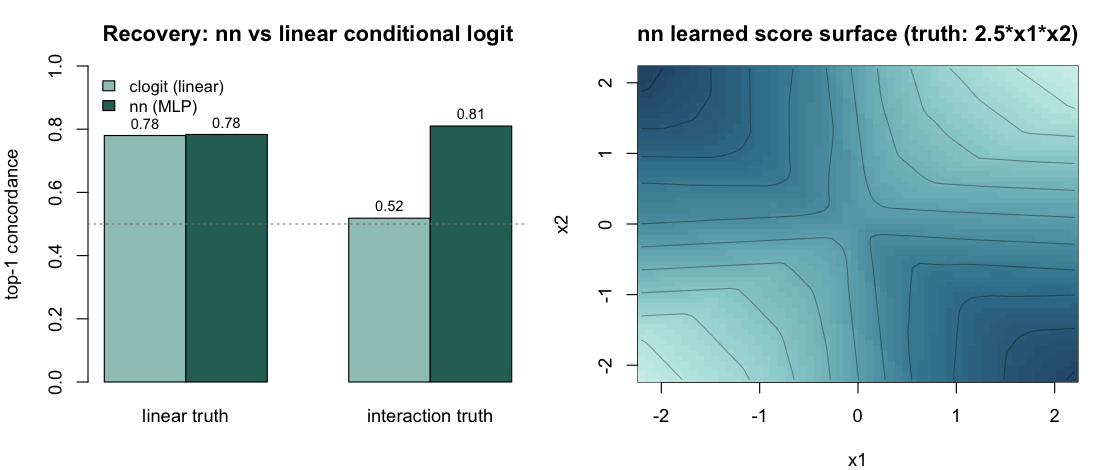
\includegraphics[width=0.9\linewidth]{figs/exp6-nn.png}
  \caption{Neural backend (experiment E6). Left: top-1 concordance of the
    \texttt{nn} MLP versus the linear \texttt{clogit} under a linear truth (tie
    at $0.78$) and a multiplicative interaction truth ($0.81$ vs $0.52$).
    Right: the learned score surface over $(x_1, x_2)$, recovering the
    opposite-sign corners of the interaction. Concordance figures are in-sample.}
  \label{fig:exp6-nn}
\end{figure}

\subsection{One front-end, one object contract}
\label{sec:framework-contract}

All three backends return an object of class \texttt{rem}: a list holding the
fitted model in \texttt{\$fit}, the chosen \texttt{method}, the original
\texttt{formula}, the parsed terms, and the number of observations. The shared
S3 methods (\code{print()}, \code{summary()}, \code{coef()}, \code{plot()},
\code{logLik()}, \code{predict()}) delegate to \texttt{\$fit}, so downstream code
is written once against the \texttt{rem} contract regardless of backend; the
\texttt{nn} fit carries its own inner methods (for instance the
partial-dependence plot) to which the outer \texttt{rem} methods forward. A
minimal end-to-end call looks as follows.

\begin{verbatim}
set.seed(1)
## long case-control layout (one row per candidate): clogit / nn
d <- simulate_relational_events(
  n_events = 300,
  senders = paste0("a", 1:12), receivers = paste0("a", 1:12),
  n_controls = 1, endogenous_stats = "reciprocity_count",
  endogenous_effects = c(reciprocity_count = 0.6))

## wide case-1-control layout (one row per event): gam
w <- simulate_relational_events(
  n_events = 300,
  senders = paste0("a", 1:12), receivers = paste0("a", 1:12),
  n_controls = 1, endogenous_stats = "reciprocity_count",
  endogenous_effects = c(reciprocity_count = 0.6), wide = TRUE)

## linear conditional logit
fit_cl <- rem(event ~ reciprocity_count, data = d, method = "clogit")

## smooth / time-varying via mgcv
fit_gam <- rem(~ tv(reciprocity_count), data = w, method = "gam", time = "time")

## neural conditional logit
fit_nn <- rem(event ~ reciprocity_count, data = d, method = "nn",
              nn = nn_control(hidden = c(16, 8), seed = 1))
summary(fit_nn)
plot(fit_nn$fit, type = "pdp")
\end{verbatim}

Each backend consumes the case--control data in the layout it expects:
\texttt{gam} the wide, one-row-per-event frame (\texttt{wide = TRUE}, carrying
event-minus-control difference columns), and \texttt{clogit} and \texttt{nn} the
long, one-row-per-candidate frame (carrying a 0/1 event indicator and a
stratum). Both layouts are produced by the same source---the package's own
simulator, or \pkg{eventnet}---so the user chooses linear, smooth, or neural by
switching a single \texttt{method} argument, and reads the result through one
object interface.

\section{Software design}
\label{sec:software}

\pkg{amore} is organised as a single pipeline whose stages each correspond to a
small set of exported functions: \emph{canonicalise} an event log,
\emph{sample} non-events, \emph{compute} endogenous statistics, \emph{fit} a
model, and \emph{check} the fit. The same pipeline runs in two directions --- a
simulation module generates synthetic event streams in the package's own
canonical form, so simulated and observed data flow through the identical
downstream machinery. This section walks through the stages in order, documents
the \code{rem} S3 contract that unifies the three estimation backends, describes
the goodness-of-fit family (which is restricted to the linear case-control fit),
catalogues the nine bundled datasets, and closes with a worked end-to-end
example on \code{classroom\_events}.

\subsection{Preprocessing}
\label{sec:software-preprocess}

\paragraph{Canonicalisation.}
\code{standardize\_event\_log()} maps an arbitrary event table to the package's
\code{amore\_event\_log} contract: three columns \code{sender}, \code{receiver},
\code{time}, with \code{sender}/\code{receiver} coerced to character and
\code{time} to numeric. The source column names are configurable
(\code{sender\_col}, \code{receiver\_col}, \code{time\_col}), and switches
control sorting by time, dropping of incomplete rows (\code{drop\_nas}),
self-loops (\code{drop\_loops}), duplicate \((s,r,t)\) triples
(\code{remove\_duplicates}), and a strict-monotonic-time assertion
(\code{strictly\_increasing\_time}); \code{keep\_extra} preserves any additional
covariate columns. The returned object carries the \code{amore\_event\_log}
class so that downstream functions can recognise a canonicalised log. A
companion \code{attach\_static\_covariates()} joins per-actor attribute tables
onto the stream.

\paragraph{Non-event sampling.}
Fitting a relational event model by the case-control device requires, for each
observed event (the \emph{case}), one or more non-events (the \emph{controls})
drawn from the risk set \citep{lerner2020}. \code{sample\_non\_events()}
implements this with three orthogonal axes. The \code{scope} argument fixes the
candidate pool: \code{"all"} uses every actor observed in the log,
\code{"appearance"} restricts to actors already present by the focal time, and
\code{"citation"} restricts receivers to previously active targets. The
\code{mode} argument selects the design (\code{"one"} matched-set vs.\
\code{"two"} permuted), and \code{risk} governs the risk set itself:
under \code{risk = "remove"} a dyad is dropped from its own control pool once it
has fired (and any dyad firing at the focal timestamp is treated as a concurrent
event, not an eligible non-event), which is the correct convention for
non-repeatable processes such as species invasion. Structurally ineligible
dyads can be excluded wholesale through \code{exclude\_pairs}, a two-column
\((\text{sender}, \text{receiver})\) table. The number of controls per case is
\code{n\_controls}, and \code{seed} makes the draw reproducible.

\paragraph{Endogenous features.}
\code{compute\_endogenous\_features()} computes the requested statistics on the
sampled case-control table. The key semantic subtlety is that controls must read
the \emph{true} network history without themselves polluting it: a sampled
non-event that never occurred should not update degrees, reciprocity, or recency
state for later rows. This is handled by the \code{history\_log} argument. When
the true event log is passed as \code{history\_log}, only rows whose
\((\text{sender}, \text{receiver}, \text{time})\) triple appears in that log
update the running network state, while all other rows (the sampled controls)
have their statistics computed against that state but never enter it. The
default catalogue is \code{c("sender\_outdegree", "receiver\_indegree",
"reciprocity", "recency")}; \code{half\_life} parameterises the exponentially
weighted recency variants. The full catalogue comprises 74 numeric statistics
plus the \code{sender\_receivers\_set} list-column, which returns, per row, the
set of receivers the row's sender has previously reached (joined downstream to an
external lookup to build set-valued covariates). Of the 74 numeric statistics,
66 are computed by a C++ fast path and 8 are pure-R fallbacks; the
\code{cpp\_supported\_stats()} helper reports which statistics the compiled
engine handles. The \code{history\_log} semantics are honoured natively only on
the C++ path; the R fallback raises an error if \code{history\_log} is supplied
for an R-only statistic. A \code{widen\_case\_control()} reshaper converts a long
case-\(k\)-control table to the wide case-1-control layout used by the \code{gam}
backend, emitting \code{<cov>\_ev}, \code{<cov>\_nv}, and \code{d\_<cov>}
(event-minus-control) columns; the 0/1 indicator and stratum columns are
auto-detected (the package's own \code{event} column, or \code{eventnet}'s
\code{IS\_OBSERVED}) when not named explicitly.

\subsection{Simulation}
\label{sec:software-simulation}

The simulation module generates event streams from a specified intensity and
returns them in the same canonical form the fitter consumes, so a simulated log
can be passed directly to \code{sample\_non\_events()} or, with \code{wide =
TRUE}, straight into \code{rem()}. Two engines share a single endogenous-state
machine: an exact Gillespie sampler and an approximate \(\tau\)-leap sampler
that trades exactness for speed and converges to the exact process only as the
leap interval shrinks. Both are pure R. The teaching simulators for
time-varying non-linear and hyper-event models attach the ground-truth
generating functions as an attribute on the returned object, so that recovery
experiments can compare estimates against the truth that produced the data
(Section~\ref{sec:validation}).

\subsection{The \code{rem()} fitter and its S3 contract}
\label{sec:software-rem}

\code{rem()} is the unified front-end. It takes a formula, a preprocessed
case-control \code{data} frame, and a \code{method}, and dispatches to one of
three backends:

\begin{verbatim}
rem(formula, data, method = c("gam", "clogit", "nn"),
    case = NULL, stratum = NULL, time = NULL,
    k = NULL, gam_method = NULL, nn = nn_control(), ...)
\end{verbatim}

The \code{"clogit"} backend fits a conditional logistic regression on a
case-\(k\)-control design via \code{survival::clogit()}, with strata taken from
\code{stratum} or derived as \code{cumsum(case == 1)} for the blocked
case-then-controls layout. The \code{"nn"} backend fits a multilayer perceptron
that scores every candidate in a stratum and is trained on the softmax over each
risk set --- this is the \emph{same} risk-set conditional-logistic partial
likelihood that \code{clogit} maximises, with a learned non-linear intensity in
place of the linear predictor. The \code{"gam"} backend is different in kind: it
fits the algebraically-related \emph{degenerate} case-1-control binomial
logistic regression of \citet{boschi2025rhem}, in which the response is the
constant \(1\) and the linear predictor is built from event-minus-control
differences. It does not form risk-set strata or a softmax; it coincides with a
two-element conditional logit only under a single matched control. The
\code{gam} backend is therefore the route to smooth, time-varying, non-linear,
and random-effect terms, which the formula expresses as \code{tv(x)},
\code{nl(x)}, \code{tvnl(x)}, and \code{re(x)} respectively, delegating to
\code{mgcv}.

All three backends return an object of class \code{"rem"} --- a list holding the
underlying fit (\code{\$fit}), the \code{method}, the \code{formula}, the parsed
\code{terms}, and the observation count \code{n}. The S3 methods delegate to the
inner fit object: \code{print.rem()} reports the method, formula, and \(n\);
\code{summary.rem()}, \code{coef.rem()}, \code{plot.rem()},
\code{logLik.rem()}, and \code{predict.rem()} forward to the backend's
corresponding method. For \code{method = "nn"} there is deliberately no
coefficient table --- \code{coef()} returns \code{NULL}, \code{summary()}
reports in-sample (and, with a validation split, held-out) concordance, and
\code{plot(type = "pdp")} draws per-feature partial-dependence curves. The
neural backend is pure R with no extra dependencies, its analytic gradients
hand-derived and verified against numerical differentiation; it accepts
numeric covariates only and provides no uncertainty quantification.
Architecture and training are configured through \code{nn\_control()}
(hidden-layer sizes, activation, epochs, Adam learning rate, L2 penalty,
validation fraction and early-stopping patience, feature standardisation, and
seed). Besides the joint multilayer perceptron, \code{nn\_control(architecture
= "additive\_spline", spline\_df, batch\_strata)} selects the additive
B-spline architecture of Section~\ref{sec:framework-nn-additive}: per-covariate
basis expansions under a single linear layer, trained on the same partial
likelihood, with optional mini-batching over strata for large event logs. Dependency posture is deliberately light: \code{survival} and
\code{Rcpp} are Imports, while \code{mgcv} is only suggested and the \code{gam}
backend raises an informative error at call time if it is absent.

\subsection{Goodness of fit}
\label{sec:software-gof}

\pkg{amore} ships the cumulative martingale-residual goodness-of-fit family of
\citet{boschi2025gof}. Each entry point builds, through a shared internal routine, a single
case-control sample (drawn at \code{n\_controls = 1}, the paper's NCC \(m=2\)
setup) and a single fitted partial-likelihood model:
\code{gof\_univariate()} tests one covariate via the supremum of the normalised
cumulative score process, whose null distribution is a standard Brownian bridge,
so its p-value follows the Kolmogorov--Smirnov series;
\code{gof\_multivariate()} tests a \(q\)-dimensional smooth or random-effect
term against a \(q\)-dimensional Brownian bridge with an empirical (simulated)
p-value; \code{gof\_global()} forms a Cauchy-combination omnibus statistic with
an analytic p-value; and \code{gof\_auxiliary()} runs a multiplier Monte Carlo
test. A standalone \code{martingale\_residuals()} returns the per-row residuals
for diagnostic plotting.

The single most important scoping fact is that \textbf{this family supports the
linear case-control fit only}. All four entry points route through an internal
fitter that fits a no-intercept binomial GLM on case-minus-control differences
and hard-rejects any effect specification other than \code{"linear"}:

\begin{verbatim}
bad <- model != "linear"
if (any(bad)) {
  stop("Only effect type \"linear\" is supported here. Got: ",
       paste(unique(model[bad]), collapse = ", "))
}
\end{verbatim}

Internally the cumulative residual process is re-centred by subtracting a linear
ramp so that it ends at zero at the maximum-likelihood estimate --- a heuristic
alignment to the score-subtraction step of the Boschi--Wit construction --- and
the number of matched controls is fixed at one. These are the relevant
limitations: the GOF family does not yet cover non-linear or time-varying fits,
nor \(m>2\) nested case-control designs.

\subsection{Bundled datasets}
\label{sec:software-data}

The package ships nine documented data objects spanning roughly two orders of
magnitude in event count (Table~\ref{tab:datasets}): six directed event streams,
two per-actor attribute tables, and one exogenous distance matrix. Each event
stream is built by a script under \code{data-raw/} from a public source with a
recorded DOI, and four of the streams carry the Unix epoch of \code{time = 0} as
\code{attr(., "unix\_origin")} on the data frame, allowing absolute timestamps to
be recovered. Figure~\ref{fig:datasets-rate} shows the event-rate profiles and
Figure~\ref{fig:datasets-degrees} the degree distributions across the streams.

\begin{figure}[t]
\centering
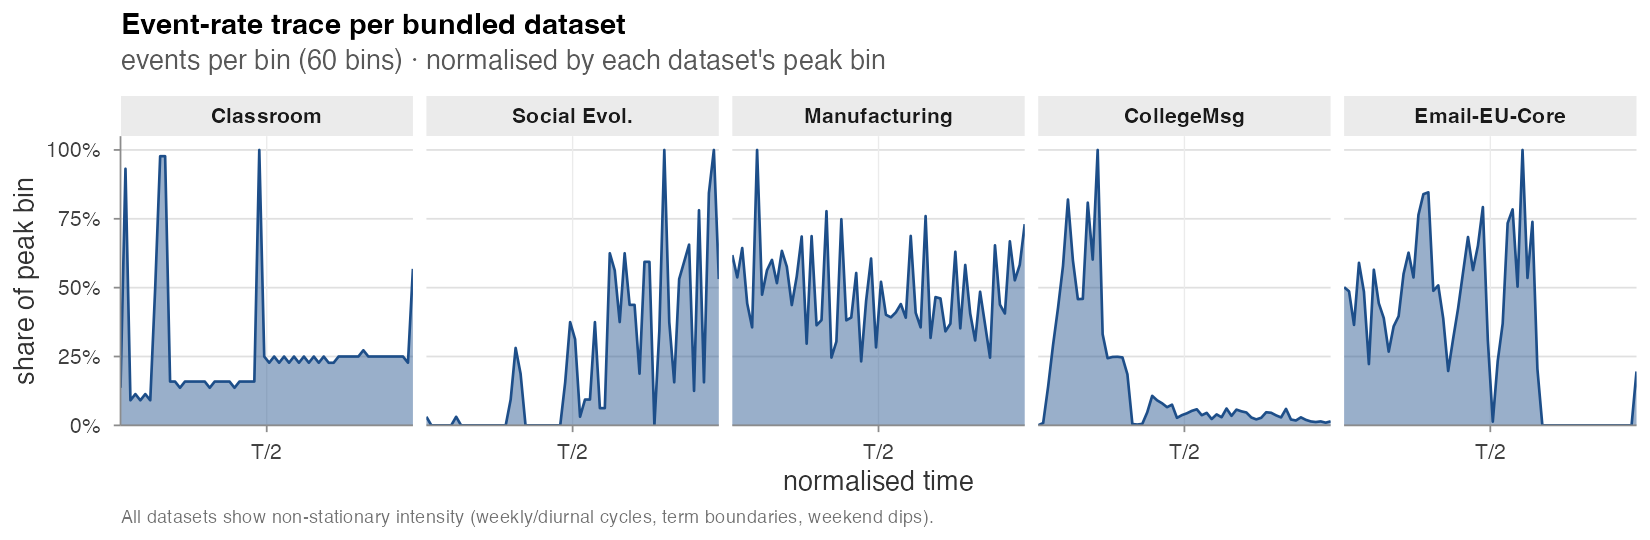
\includegraphics[width=0.8\linewidth]{figs/datasets-rate.png}
\caption{Event-rate profiles of the bundled event streams.}
\label{fig:datasets-rate}
\end{figure}

\begin{figure}[t]
\centering
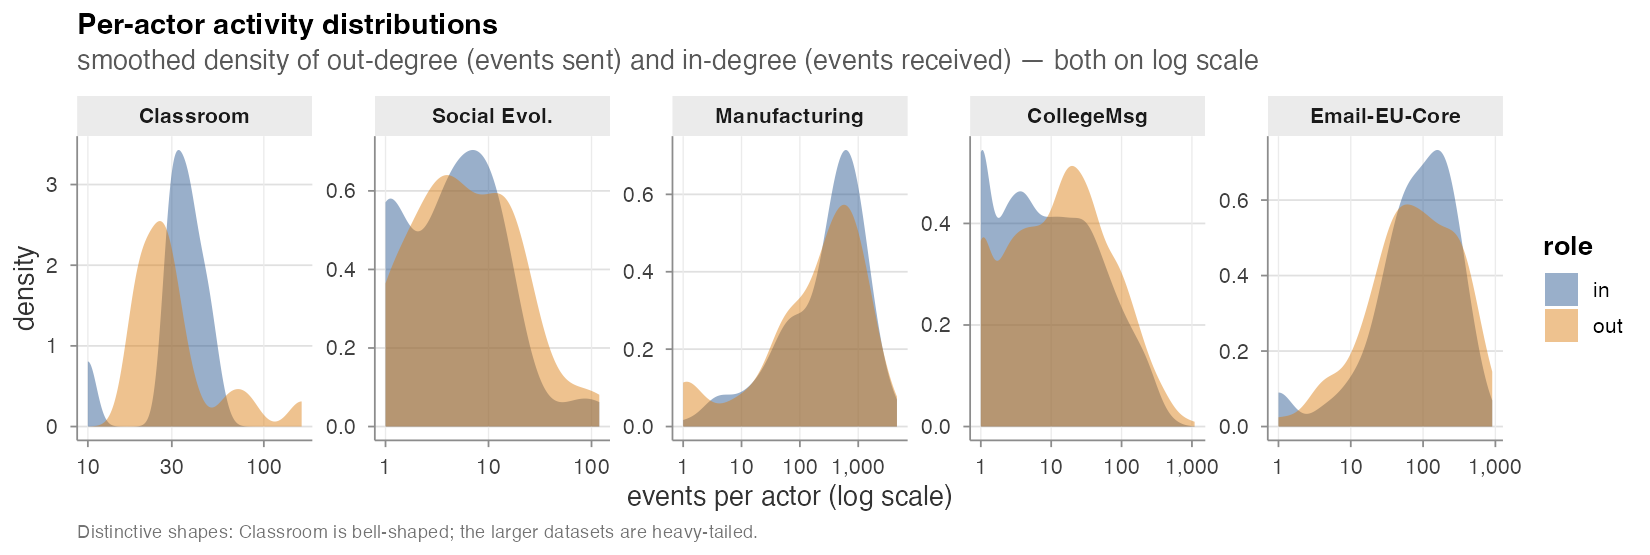
\includegraphics[width=0.8\linewidth]{figs/datasets-degrees.png}
\caption{Degree distributions across the bundled event streams.}
\label{fig:datasets-degrees}
\end{figure}

\begin{table}[t]
\centering
\caption{The nine bundled data objects. Event counts span 439 to 82{,}927
(\(\sim\)2 orders of magnitude). ``unix'' marks the four event streams that
carry \code{attr(., "unix\_origin")}.}
\label{tab:datasets}
\begin{tabular}{llrl}
\hline
Object & Kind & Rows & Source \\
\hline
\code{social\_evolution\_calls}      & event stream     & 439     & Madan et al.\ (2011), \emph{goldfish} \\
\code{classroom\_events}             & event stream     & 691     & McFarland (2001), \emph{networkDynamic} \\
\code{social\_evolution\_friendship} & event stream     & 766     & Madan et al.\ (2011), \emph{goldfish} \\
\code{email\_eu\_core}               & event stream     & 12{,}216 & Paranjape et al.\ (2017), SNAP \\
\code{college\_msg}                  & event stream     & 59{,}835 & Panzarasa et al.\ (2009), SNAP \\
\code{radoslaw\_email}               & event stream     & 82{,}927 & Michalski et al.\ (2014), Network Repository \\
\code{classroom\_actors}            & actor attributes & 20      & McFarland (2001) \\
\code{social\_evolution\_actors}     & actor attributes & 84      & Madan et al.\ (2011) \\
\code{dist\_matrix}                  & distance matrix  & 56\(\times\)56 & US Census TIGER/Line \\
\hline
\end{tabular}
\end{table}

\subsection{A worked end-to-end example}
\label{sec:software-example}

The following session takes \code{classroom\_events} --- 691 timestamped
directed interactions among 20 students \citep{McFarland2001} --- through the
full loop: sample non-events, fit a linear conditional logit, fit a smooth
counterpart, and check the fit.

\begin{verbatim}
library(amore)
data(classroom_events)

## 1. Sample one matched control per event from the full actor pool.
cc <- sample_non_events(classroom_events,
                        n_controls = 1, scope = "all", mode = "one",
                        seed = 11)

## 2. Compute endogenous statistics for cases and controls, reading the
##    true history but never letting controls update it.
feats <- compute_endogenous_features(
  cc,
  stats       = c("reciprocity_count", "transitivity_count"),
  history_log = classroom_events)

## 3a. Linear conditional logit (case-1-control => no-intercept binomial GLM).
fit <- rem(event ~ reciprocity_count + transitivity_count,
           data = feats, method = "clogit", stratum = "stratum")
coef(fit); summary(fit)

## 3b. The same data, widened, with a non-linear reciprocity effect.
w    <- widen_case_control(feats)
fitg <- rem(~ nl(reciprocity_count) + transitivity_count,
            data = w, method = "gam")
plot(fitg)                      # the fitted smooth panel

## 4. Goodness of fit of the linear specification.
m <- c(reciprocity_count = "linear", transitivity_count = "linear")
gof_univariate(classroom_events, m, "reciprocity_count", seed = 11)
gof_global(classroom_events, m, seed = 11)

## 5. Martingale residuals for diagnostic plotting.
res <- martingale_residuals(classroom_events, m, seed = 11)
plot(res$time, res$residual); abline(h = 0)
\end{verbatim}

Steps 3a and 3b illustrate the division of labour between backends: the
\code{clogit} fit gives interpretable linear coefficients on the matched
case-control strata, while the \code{gam} fit relaxes a chosen term to a smooth
on the case-1-control difference design. Steps 4 and 5 exercise the
goodness-of-fit family on the linear specification ---
Figure~\ref{fig:gof-process} shows the univariate cumulative residual process,
which starts and ends near zero under correct specification. The neural backend
is reachable from exactly the same upstream output by switching to
\code{method = "nn"} (Section~\ref{sec:validation}).

\begin{figure}[t]
\centering
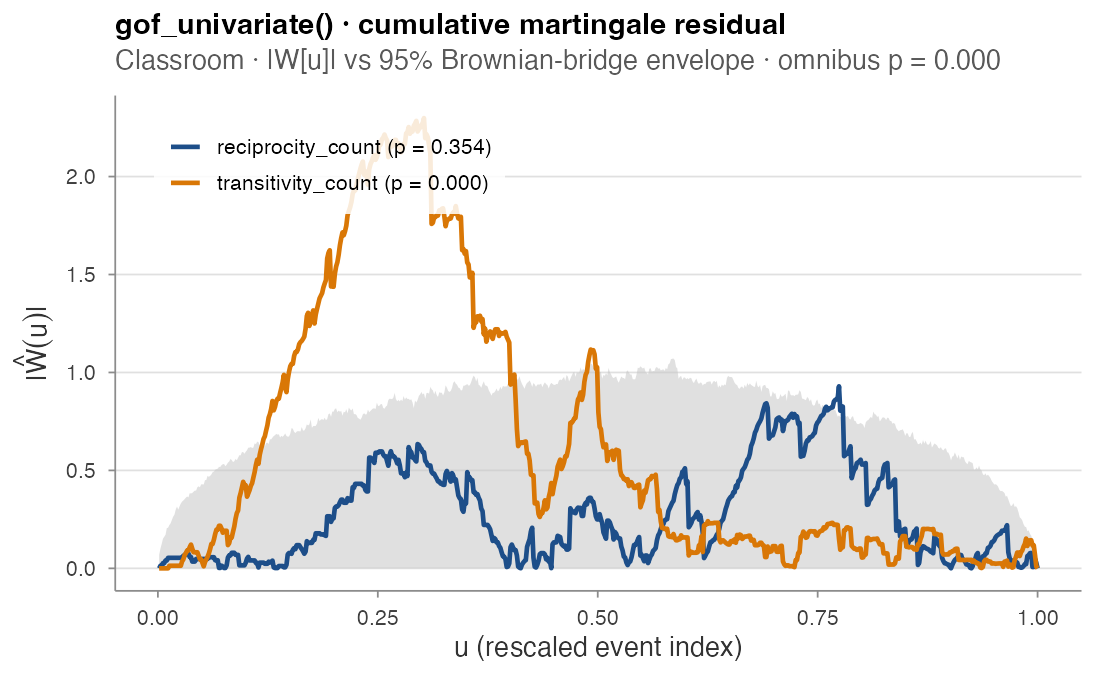
\includegraphics[width=0.7\linewidth]{figs/est-gof-process.png}
\caption{Univariate cumulative martingale-residual process for the
\code{reciprocity\_count} term on \code{classroom\_events}; under correct
specification the normalised process starts and ends near zero
\citep{boschi2025gof}.}
\label{fig:gof-process}
\end{figure}

\section{The simulation engine}
\label{sec:simulation}

A relational-event model is only as testable as the data-generating
process one can pair with it. \pkg{amore} therefore ships a first-class
forward simulator, \texttt{simulate\_relational\_events()}, alongside the
estimation machinery. The simulator is not an afterthought: it is the
ground-truth oracle behind every recovery experiment in
Section~\ref{sec:validation}, and its output is shaped so that it feeds
\texttt{rem()} without an intervening reshaping step. This section
describes the two driving algorithms (exact Gillespie and approximate
$\tau$-leap), the five generative mechanisms they compose, the
ready-to-fit case--control output, the measured scaling behaviour, and the
companion hyperedge (RHEM) simulators.

\subsection{One front door, five composable mechanisms}
\label{sec:sim-mechanisms}

\texttt{simulate\_relational\_events()} exposes a single entry point that
layers five mechanisms on top of an event-by-event inner loop. Each
mechanism is opt-in through its own arguments and the mechanisms compose
freely:

\begin{enumerate}
\item \textbf{A homogeneous baseline.} A positive \texttt{baseline\_rate}
  multiplies the hazard of every admissible dyad, giving the minimal
  memoryless process \citep{butts2008}.
\item \textbf{Per-dyad contribution logits.} A static $S \times R$ matrix
  \texttt{contribution\_logits} adds a dyad-specific term to the log-rate
  --- for example inter-state distances, role similarities, or a planted
  non-linear surface $f(x_{sr})$ (used to stress smooth recovery in
  experiment E2 of Section~\ref{sec:validation}).
\item \textbf{Exogenous actor covariates.} Per-actor numeric tables
  (\texttt{sender\_covariates}, \texttt{receiver\_covariates}) with their
  effect vectors enter the linear predictor additively. The companion
  generator \texttt{simulate\_actor\_covariates()} produces either static
  per-actor attributes or time-stamped AR(1) processes for repeated
  exogenous draws.
\item \textbf{Endogenous statistics.} Any subset of the endogenous
  catalogue (Section~\ref{sec:statistics}) can be activated through
  \texttt{endogenous\_stats} / \texttt{endogenous\_effects}; the simulator
  maintains the corresponding state matrices and updates them after every
  fired event, so the intensity of the next event depends on the realized
  history. This is the formulation of \citet{juozaitiene2024}.
\item \textbf{Time-varying global covariates.} A piecewise-constant grid
  (\texttt{global\_covariates} with a \texttt{time\_start} column, and
  \texttt{global\_effects}) rescales the total event rate by
  $\exp\!\big(\sum_k \beta_k\, x_k(t)\big)$. Because the multiplier is the
  same for every dyad, it cancels from the per-dyad selection
  probabilities and acts only on the waiting-time distribution --- the
  identifiability structure exploited by the time-shift sampling of
  \citet{lembo2025}.
\end{enumerate}

The same five-mechanism state machine drives both algorithms, so a model
specified once can be simulated under either scheme without change.

\subsection{Gillespie and \texorpdfstring{$\tau$}{tau}-leap}
\label{sec:sim-algorithms}

The default algorithm is the exact event-driven Gillespie scheme
\citep{gillespie1977}: at each step the simulator computes every dyad's
current intensity, draws the inter-event waiting time from an exponential
with rate equal to the sum of all dyadic intensities, and selects the
firing dyad with probability proportional to its intensity (a softmax over
the risk set). Because the full risk set is recomputed after every event,
Gillespie is exact but per-event in cost.

When global covariates are active the simulator switches to a
\emph{boundary-aware} Gillespie variant: whenever a sampled waiting time
would carry the clock across an interval boundary of the
piecewise-constant grid, the clock is advanced to the boundary without
recording an event and the next waiting time is redrawn under the new
global multiplier. This keeps the inhomogeneous process exact rather than
approximating it on the grid.

The alternative is \texttt{method = "tau\_leap"}, a time-driven
approximation. It advances the clock by a fixed step $\tau$ and, for every
dyad, draws a $\mathrm{Poisson}(\lambda_{sr}(t)\,\tau)$ number of events
using the rates at the \emph{start} of the step; events that fire within a
step are placed at uniform times in $[t, t+\tau)$, reported in time order,
and share the start-of-step state, which is then updated once at the end
of the step. The $\tau$-leap scheme trades exactness for predictable,
vectorised work per step and is stated honestly as an approximation: it
converges in distribution to the exact Gillespie result only as
$\tau \to 0$. Practical use requires $\lambda\tau \ll 1$ on every active
dyad and $\tau$ smaller than the shortest global-covariate interval
(within-step boundary crossings are not resolved).

\subsection{Risk-set rule and ready-to-fit output}
\label{sec:sim-output}

Two further controls make the simulator a direct estimation companion
rather than a bare event generator.

\textbf{Risk-set rule.} \texttt{risk = "standard"} (the default) keeps
every dyad eligible at every step. \texttt{risk = "remove"} drops a dyad
from the risk set as soon as it fires, mimicking one-shot processes such
as species invasions or first-citation events, where a dyad cannot repeat.

\textbf{Case--control output.} Setting \texttt{n\_controls = k} emits a
stratified case--control table directly: each realized event becomes one
\emph{case} row paired with $k$ \emph{control} rows sampled from the
non-event risk set at that moment, all sharing a \texttt{stratum}
identifier, with an \texttt{event} indicator (1 for the case, 0 for
controls). When endogenous statistics or global covariates are active, the
value each row's dyad carried at its event time is appended as a column,
so a downstream conditional-logistic or GAM fit recovers the planted
effects. This is the sampled-risk-set reduction of \citet{lerner2020}
produced at generation time.

For the common case-1-control design, \texttt{wide = TRUE} (which requires
\texttt{n\_controls = 1}) reshapes the long table to one row per event,
carrying the event-dyad actors (\texttt{sender\_ev},
\texttt{receiver\_ev}), the matched control-dyad actors
(\texttt{sender\_nv}, \texttt{receiver\_nv}), and for each covariate the
event value (\texttt{<cov>\_ev}), the control value (\texttt{<cov>\_nv}),
and their difference (\texttt{d\_<cov>}). The difference columns are
exactly the design matrix of the degenerate case-1-control logistic
regression fitted by the \texttt{gam} backend
(Section~\ref{sec:framework}), so the simulator's output is ready to fit
with no further preparation:

\begin{verbatim}
wide_events <- simulate_relational_events(
  n_events           = 5,
  senders            = LETTERS[1:3],
  receivers          = LETTERS[1:3],
  n_controls         = 1,
  endogenous_stats   = "reciprocity_count",
  endogenous_effects = c(reciprocity_count = 0.6),
  wide               = TRUE)
\end{verbatim}

\subsection{Scaling: when to leap}
\label{sec:sim-scaling}

Experiment E4 of Section~\ref{sec:validation} times both algorithms over a
$4 \times 5 \times 2$ grid
(\texttt{n\_actors} $\in \{15, 30, 60, 100\}$,
\texttt{n\_events} $\in \{500, 1000, 2500, 5000, 10000\}$, both methods,
$\tau = 0.05$), on a single reciprocity term with no case--control
sampling so the wall-clock isolates the simulator. Absolute seconds are
machine-specific (Apple Silicon M1 Max); the scaling shape and ratios are
what transfer.

On the stable cells, $\tau$-leap is \textbf{22--42$\times$ faster than
Gillespie at \texttt{n\_actors} $= 60$} and \textbf{37$\times$ to
$\approx 100\times$ faster at \texttt{n\_actors} $= 100$}, the gap widening
with \texttt{n\_events} (Gillespie recomputes the full risk set per event;
$\tau$-leap takes vectorised Poisson leaps). At 10,000 events the
100-actor cell runs in $\approx 3.4$\,s under Gillespie and
$\approx 0.033$\,s under $\tau$-leap. Figure~\ref{fig:exp4-scaling}
plots the full grid.

\begin{figure}[t]
\centering
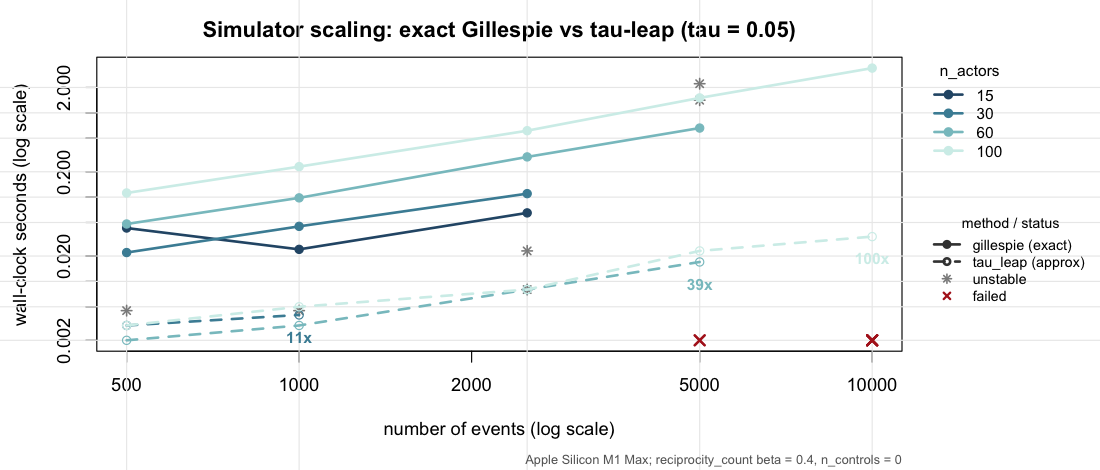
\includegraphics[width=0.9\textwidth]{figs/exp4-scaling.png}
\caption{Simulator wall-clock scaling (experiment E4). $\tau$-leap
(dashed) bundles events into fixed time slices and scales markedly better
than the exact per-event Gillespie scheme (solid) as the actor universe
grows, reaching $\approx 100\times$ at 100 actors and 10{,}000 events.
Absolute times are machine-specific; the ratios transfer. Cells that fall
in the small-network failure regime are omitted.}
\label{fig:exp4-scaling}
\end{figure}

We report the failure regime as plainly as the speed-ups, because both
back-ends break down at \emph{small} \texttt{n\_actors} under a strongly
self-exciting reciprocity process, for opposite reasons. Gillespie's
per-dyad softmax underflows (``too few positive probabilities'') at
\texttt{n\_actors} $\in \{15, 30\}$ for \texttt{n\_events} $\ge 5000$ (and
at 60 actors for 10,000 events): the self-excitation concentrates almost
all probability mass on a few reciprocating dyads, and the remaining
intensities round to zero. The $\tau$-leap intensities instead explode
into a memory blow-up (seed-dependent at small sizes; all replicates fail
at 10,000 events for \texttt{n\_actors} $\le 60$). At 10,000 events only
the 100-actor cell is clean for both methods. The practical guidance is
to use Gillespie for small or dense networks where exactness is cheap, to
use $\tau$-leap for large actor universes where wall-clock matters, and in
the high-rate small-network corner to reduce the self-exciting effect
size, raise the actor count, or validate $\tau$ against a short Gillespie
run before trusting it. None of these limits is silent: each failure
surfaces as an error rather than a wrong number.

\subsection{Hyperedge and RHEM simulators}
\label{sec:sim-hyperedge}

For relational \emph{hyper}-events --- where senders and receivers are
\emph{sets} of actors rather than single actors --- \pkg{amore} ships three
companion simulators that follow the formulation of
\citet{boschi2025rhem}. \texttt{simulate\_hyperedge\_events()} generates
\emph{undirected} multi-actor meetings (subsets of the actor set of size up
to \texttt{max\_size}), matching Section~4 of that paper.
\texttt{simulate\_directed\_hyperedge\_events()} generates \emph{directed}
two-mode hyperevents from a sender set $I_m$ to a receiver set $J_m$ (both
non-empty), the data model of Section~5 for citation networks. Both fire a
candidate hyperedge $(I, J)$ with rate
$\lambda(t, I, J) = \lambda_0 \exp\!\big(\sum_k \beta_k\, x_k(t, I, J)\big)$
and draw waiting times from an exponential with the total intensity ---
the same Gillespie logic as the dyadic engine, lifted to set-valued
events. The supported hyperedge statistics are the cardinality terms
(\texttt{size}, \texttt{size\_I}, \texttt{size\_J}), past-event
\texttt{activity}, and directed/undirected \emph{subset repetition}
\texttt{subrep\_<$\rho$>} (paper eq.~4), the mechanism by which a recurring
subset of participants raises the rate of future hyperedges that contain
it. Figure~\ref{fig:hyper-running-subrep} illustrates a subset-repetition
driven directed hyperevent stream.

Because each step enumerates every candidate hyperedge, the candidate
space is exponential in the universe size; these simulators are therefore
explicitly bounded to small actor / item universes (practically
$|V| \le 20$ with small maximum cardinality), and the documentation states
this limit. The third simulator,
\texttt{simulate\_directed\_hyperevents\_tvnl()}, is a teaching-oriented
generator with a \emph{time-varying} sender effect $\alpha(t)$ and a
\emph{non-linear} receiver effect $f(x)$, intended for demonstrating
GAM-based recovery of smooth (TV/NL) effects. It attaches the ground-truth
$\alpha(t)$ and $f(x)$ as \texttt{attr(., "truth")} on its output so a
fitted smooth can be compared directly against the function that generated
it.

\begin{figure}[t]
\centering
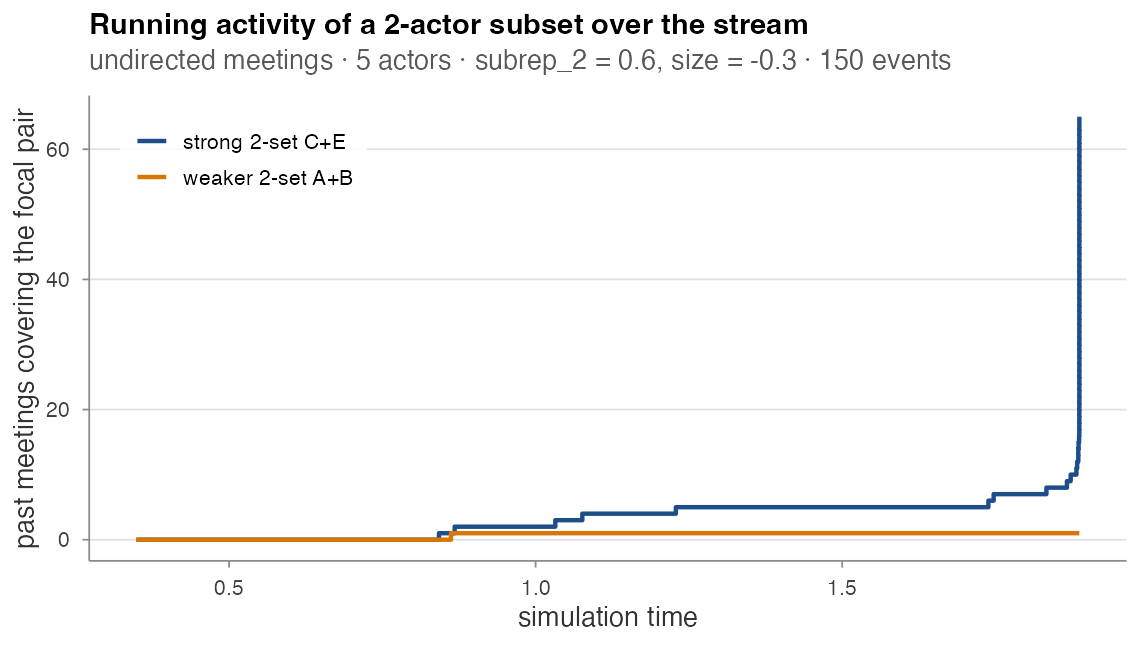
\includegraphics[width=0.7\textwidth]{figs/hyper-running-subrep.png}
\caption{A directed hyperevent stream simulated under a positive subset
repetition (\texttt{subrep}) effect: recurring participant subsets raise
the intensity of future hyperedges that contain them
\citep{boschi2025rhem}. The hyperedge simulators reuse the dyadic engine's
Gillespie logic over set-valued candidates.}
\label{fig:hyper-running-subrep}
\end{figure}

The hyperedge simulators produce hyperedge logs and case--control
hyperedge features; they exercise the full RHEM feature path. We note for
honesty that no bundled vignette yet carries a hyperedge stream all the way
through an end-to-end \texttt{rem()} fit --- the RHEM features are
\texttt{rem}-ready but the closed-loop demonstration on hyperevent data is
left to future work.

\section{Validation}
\label{sec:validation}

Correctness in \pkg{amore} rests on two complementary layers. The first is
the automated test suite that ships with the package --- several thousand
assertions covering the case-control reshaping, the
endogenous-statistics engine, each of the three \code{rem()} backends, the
simulation kernels, and the goodness-of-fit family. The second layer, and
the subject of this section, is a battery of six end-to-end experiments
(E1--E6) that probe distinct correctness properties of the simulator and the
estimation pipeline as a whole. Each experiment fixes a known ground truth,
runs the full toolchain, and compares the recovered quantity against that
truth. The numbers reported below are fresh runs (June 2026) and reproduce
the corresponding entries in the package's \texttt{validation-experiments}
article. We frame these as quality-assurance sign-and-scale checks rather
than as a formal bias/variance study; where an effect is a genuine
finite-sample artifact rather than a defect, we say so.

Two of the experiments correct conclusions drawn in earlier internal runs.
E3 finds that the naive stratified conditional logit is already robust to
extreme sender-activity heterogeneity, so the Gamma frailty that an earlier
reading deemed necessary is in fact unnecessary in this setting. E5 finds
that a previously reported simulator/post-hoc ``ordering bug'' was a
comparison artifact: once the recompute is aligned to the simulator's
history semantics, parity holds to floating-point precision. We present both
corrections explicitly, because the cross-implementation oracle that exposed
them is itself a deliverable of the package.

\subsection{E1: Recovery of a linear endogenous effect}
\label{sec:val-e1}

The first property is internal consistency between the simulator and the
case-control partial likelihood: a coefficient $\beta$ planted in
\code{simulate\_relational\_events()} should be recovered, up to Monte Carlo
noise, by a stratified \code{clogit} fit on the emitted case-control table.
The design uses a single endogenous term, \texttt{reciprocity\_count}, on a
15-actor one-mode network with 800 events per replicate and one control per
case. Five targets $\beta \in \{-0.4, 0, 0.4, 0.8, 1.2\}$ (the last a
deliberate stress row) are each replicated 30 times, for 150 fits.

\begin{table}[ht]
\centering
\caption{E1 linear recovery. Estimates are essentially unbiased for small
and moderate $\beta$; bias grows with effect strength. Wald coverage sits
between 0.90 and 1.00.}
\label{tab:val-e1}
\begin{tabular}{rrrrrr}
\hline
$\beta_{\text{true}}$ & mean est & bias & emp.\ SD & mean Wald SE & 95\% coverage \\
\hline
$-0.4$        & $-0.395$ & $+0.005$ & $0.046$ & $0.043$ & $0.97$ \\
$0.0$         & $-0.004$ & $-0.004$ & $0.037$ & $0.036$ & $0.93$ \\
$0.4$         & $0.406$  & $+0.006$ & $0.086$ & $0.067$ & $0.90$ \\
$0.8$         & $0.851$  & $+0.051$ & $0.201$ & $0.221$ & $1.00$ \\
$1.2$ (stress)& $1.347$  & $+0.147$ & $0.467$ & $0.455$ & $0.97$ \\
\hline
\end{tabular}
\end{table}

Table~\ref{tab:val-e1} reports the outcome. The estimator is essentially
unbiased for $|\beta| \le 0.4$ (bias $\le 0.006$); the bias then grows with
effect strength, reaching $+0.051$ at $\beta = 0.8$ and $+0.147$ at the
$1.2$ stress row. This is a real finite-sample effect, not a defect: at high
reciprocity the events concentrate on a few reciprocating dyads, and an
800-event log becomes informationally limited. Wald coverage lies between
0.90 and 1.00 across cells; at $\beta = 0.4$ the empirical SD ($0.086$)
exceeds the mean Wald SE ($0.067$), so the interval is mildly
anticonservative there. Two of the 150 fits emitted \code{clogit}
convergence warnings (the extreme replicates in the high-$\beta$ cells);
their estimates are retained. Figure~\ref{fig:val-e1} shows the
per-cell estimate distributions.

\begin{figure}[ht]
\centering

\includegraphics[width=0.9\textwidth]{figs/exp1-recovery.png}
\caption{E1 recovery distributions of $\hat\beta$ across the five target
values; the spread widens with the planted effect.}
\label{fig:val-e1}
\end{figure}

\subsection{E2: Recovery of a non-linear smooth effect}
\label{sec:val-e2}

The second experiment tests whether a non-linear dyad-level effect, injected
through the simulator's \texttt{contribution\_logits} matrix, is recovered in
shape by a penalized-spline conditional logit. A static dyadic covariate
$x_{sr} \sim \mathrm{Uniform}(0, 6)$ is placed on an 18-actor network with
true contribution $f(x) = \sin(x) - 0.3(x - 3)$. The simulator runs for
1{,}500 events with three controls per case, and
\code{clogit(event \textasciitilde{} pspline(x, df = 6) + strata(stratum))}
extracts the partial smooth on a 150-point grid. After centering both curves,
the centred RMSE is \textbf{0.075} and the Pearson correlation between the
estimated and true curves is \textbf{0.998}. The penalized-spline
\code{clogit} therefore recovers the injected shape with high fidelity
(Figure~\ref{fig:val-e2}).

\begin{figure}[ht]
\centering
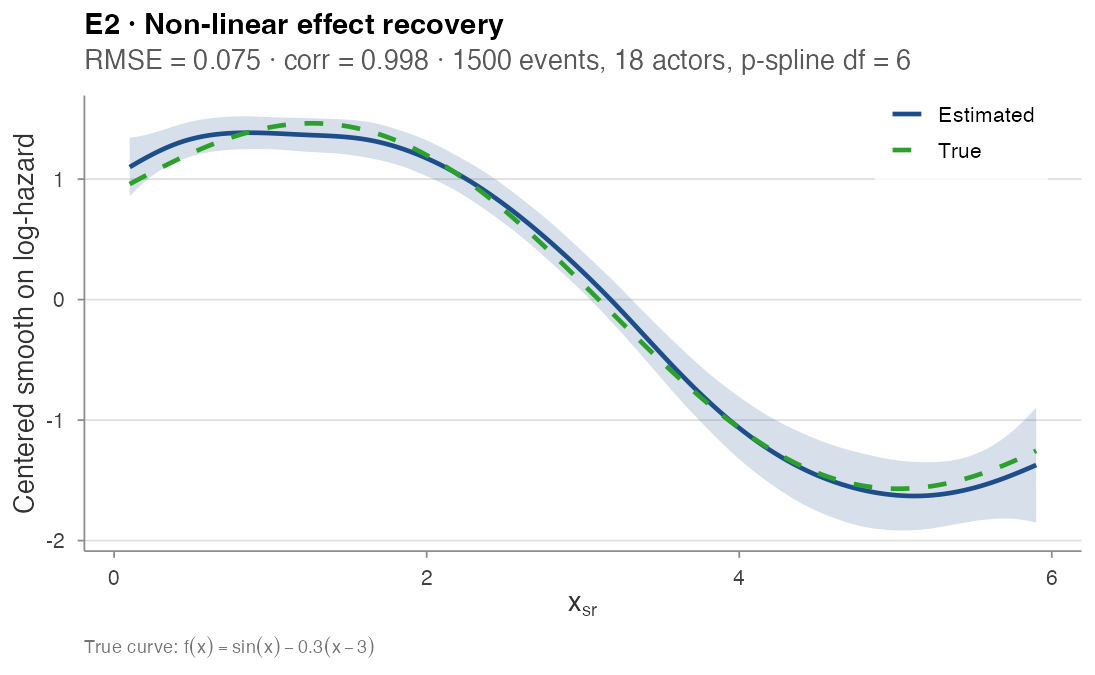
\includegraphics[width=0.7\textwidth]{figs/exp2-smooth.png}
\caption{E2 smooth recovery: the estimated penalized-spline partial effect
(with confidence band) overlaid on the true $f(x) = \sin(x) - 0.3(x-3)$;
centred RMSE $= 0.075$, correlation $= 0.998$.}
\label{fig:val-e2}
\end{figure}

\subsection{E3: Sender frailty under activity heterogeneity}
\label{sec:val-e3}

The third experiment asks whether strong per-sender activity heterogeneity
biases a fixed-coefficient \code{clogit} on \texttt{reciprocity\_count}, and
whether a Gamma sender frailty corrects any such bias. On a 20-actor network
with true $\beta = 0.5$ and three controls per case, per-sender baseline
offsets are injected through \texttt{contribution\_logits} rows under two
heterogeneity regimes: a \emph{strong} regime with lognormal activity
(median max/min ratio $\approx 84\times$, 2{,}500 events, 8 replicates) and
a \emph{mild} regime with $\mathrm{Gamma}(2,1)$ activity ($\approx 22\times$,
1{,}500 events, 10 replicates). Each replicate fits the naive
\code{clogit(event \textasciitilde{} reciprocity\_count + strata(stratum))}
against a \code{coxph} model adding \code{frailty(sender, "gamma")}.

\begin{table}[ht]
\centering
\caption{E3 sender frailty. The naive case-control estimator is robust to
$\approx 84\times$ sender-activity heterogeneity; the Gamma frailty adds
bias and variance rather than removing it.}
\label{tab:val-e3}
\begin{tabular}{llrrr}
\hline
Regime & Spec & mean $\hat\beta$ & SD & bias \\
\hline
strong ($\approx 84\times$) & naive clogit      & $0.498$ & $0.100$ & $-0.002$ \\
                            & $+$ sender frailty & $0.539$ & $0.110$ & $+0.039$ \\
mild ($\approx 22\times$)   & naive clogit      & $0.539$ & $0.086$ & $+0.039$ \\
                            & $+$ sender frailty & $0.554$ & $0.140$ & $+0.054$ \\
\hline
\end{tabular}
\end{table}

The hypothesized failure mode does not manifest
(Table~\ref{tab:val-e3}). The naive case-control estimator is robust to
sender-activity heterogeneity: in the strong regime it is essentially
unbiased ($-0.002$). Adding the Gamma frailty reduces bias in neither
regime; it introduces a small upward bias and inflates the variance, and
every frailty fit emitted inner-loop convergence warnings. The reason is
structural: the stratified case-control likelihood already conditions on the
stratum, which absorbs the per-sender baseline, so an extra frailty term has
nothing to correct and only injects noise. This \textbf{revises an earlier
reading} of the experiment, which had expected the frailty to be needed and
judged the design under-powered. With the stronger design, the conclusion is
that the correction is unnecessary in this setting
(Figure~\ref{fig:val-e3}).

\begin{figure}[ht]
\centering

\includegraphics[width=0.8\textwidth]{figs/exp3-frailty.png}
\caption{E3 frailty estimates: naive versus frailty-corrected $\hat\beta$
across replicates and regimes; the naive estimator centers on the truth.}
\label{fig:val-e3}
\end{figure}

\subsection{E4: Simulator wall-clock scaling}
\label{sec:val-e4}

The fourth experiment compares the two simulation kernels. The Gillespie
scheme is exact but processes one event at a time, recomputing the full risk
set per event; the $\tau$-leap scheme bundles events into fixed time slices
and should scale better for large actor universes. A
$4 \times 5 \times 2$ grid varies
\code{n\_actors} $\in \{15, 30, 60, 100\}$,
\code{n\_events} $\in \{500, 1000, 2500, 5000, 10000\}$, and
\code{method} $\in \{$\texttt{gillespie}, \texttt{tau\_leap}$\}$
($\tau = 0.05$), with a single reciprocity term at $\beta = 0.4$ and no
case-control sampling so wall-clock isolates the simulator. Absolute seconds
are machine-specific (Apple Silicon M1 Max); the scaling shape and the
ratios are what transfer.

\begin{table}[ht]
\centering
\caption{E4 simulator timings (stable cells). The $\tau$-leap kernel is
22--42$\times$ faster at \code{n\_actors} $= 60$ and up to
$\approx 100\times$ faster at \code{n\_actors} $= 100$.}
\label{tab:val-e4}
\begin{tabular}{rrrrr}
\hline
\code{n\_actors} & \code{n\_events} & Gillespie (s) & $\tau$-leap (s) & speedup \\
\hline
60  & 500    & $0.044$ & $0.002$ & $22\times$ \\
60  & 1{,}000  & $0.097$ & $0.003$ & $32\times$ \\
60  & 2{,}500  & $0.281$ & $0.008$ & $35\times$ \\
60  & 5{,}000  & $0.673$ & $0.016$ & $42\times$ \\
100 & 500    & $0.110$ & $0.003$ & $37\times$ \\
100 & 2{,}500  & $0.620$ & $0.009$ & $73\times$ \\
100 & 5{,}000  & $1.50$  & $0.018$ & $\approx 80\times$ \\
100 & 10{,}000 & $3.40$  & $0.033$ & $\approx 100\times$ \\
\hline
\end{tabular}
\end{table}

Table~\ref{tab:val-e4} reports the stable cells. The $\tau$-leap kernel is
22--42$\times$ faster at \code{n\_actors} $= 60$ and from 37$\times$ to
$\approx 100\times$ faster at \code{n\_actors} $= 100$, the gap widening
with \code{n\_events}. The honest counterpart is a shared failure map at
\emph{small} actor universes under this strongly self-exciting reciprocity
process: both back-ends break down, for opposite reasons. Gillespie's
per-dyad softmax underflows (``too few positive probabilities'') at
\code{n\_actors} $\in \{15, 30\}$ for \code{n\_events} $\ge 5000$ (and at 60
for 10{,}000 events), while $\tau$-leap's intensities blow up into a memory
explosion (seed-dependent at small sizes; all replicates fail at
\code{n\_events} $= 10000$ for \code{n\_actors} $\le 60$). At 10{,}000
events only the 100-actor cell is clean for both methods. This is a real
limitation worth knowing when simulating small, strongly self-exciting
networks (Figure~\ref{fig:val-e4}).

\begin{figure}[ht]
\centering
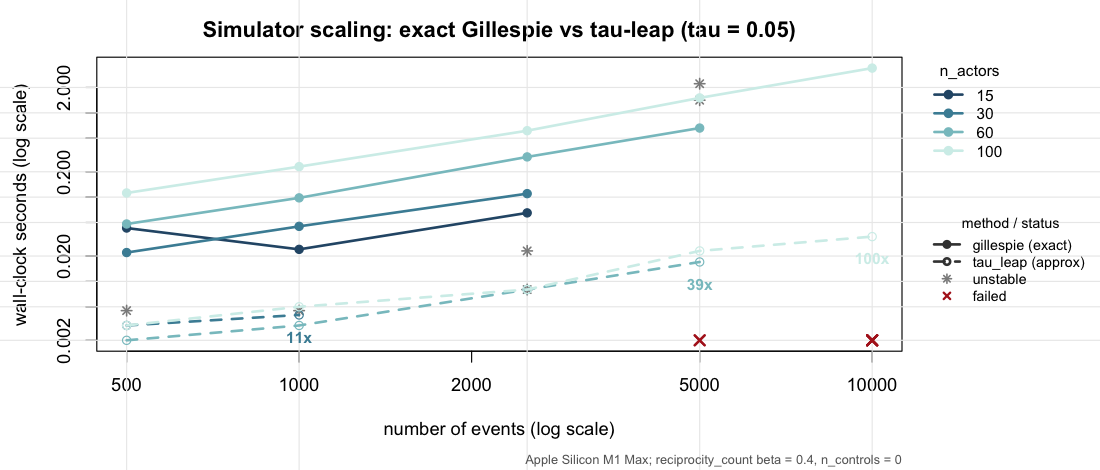
\includegraphics[width=0.8\textwidth]{figs/exp4-scaling.png}
\caption{E4 scaling lines: wall-clock seconds versus \code{n\_events} for
each kernel and actor count on log scales; $\tau$-leap stays an order of
magnitude or more below Gillespie in the stable cells.}
\label{fig:val-e4}
\end{figure}

\subsection{E5: Simulator/post-hoc engine parity}
\label{sec:val-e5}

The fifth experiment is the package's cross-implementation oracle. The
simulator records each endogenous statistic on the fly as it generates
events; the post-hoc engine \code{compute\_endogenous\_features()} re-derives
the same statistics from the timestamps alone. The two should agree
row-for-row on any case-control table the simulator emits. The design uses a
15-actor, 1{,}200-event simulation (one control per case; a 2{,}400-row
table) with 12 endogenous statistics active simultaneously across five
families and four variant axes, all C++-engine-supported. For each
statistic, \code{max |simulator - post-hoc|} is computed under two
conventions: a \emph{naive} recompute over the full case-control table, and
an \emph{aligned} recompute that passes \code{history\_log =} the realized
event rows, so that sampled controls neither pollute the running history nor
read post-update state at tied timestamps.

\begin{table}[ht]
\centering
\caption{E5 simulator/post-hoc parity. The naive recompute shows drift of
order \code{n\_events}; under \code{history\_log} alignment the engines agree
to floating-point precision.}
\label{tab:val-e5}
\begin{tabular}{lrr}
\hline
Statistic & naive (no \code{history\_log}) & aligned (\code{history\_log} $=$ events) \\
\hline
\texttt{reciprocity\_count}           & $12.0$ & $0$ \\
\texttt{transitivity\_count}          & $9.0$  & $0$ \\
\texttt{cyclic\_count}                & $10.0$ & $0$ \\
\texttt{sending\_balance\_count}      & $9.0$  & $0$ \\
\texttt{receiving\_balance\_count}    & $9.0$  & $0$ \\
\texttt{cyclic\_exp\_decay}           & $9.37$ & $4.3\times10^{-14}$ \\
\texttt{sending\_balance\_exp\_decay} & $8.67$ & $3.9\times10^{-14}$ \\
\texttt{transitivity\_time\_recent}   & $3.74$ & $0$ \\
\texttt{cyclic\_time\_recent}         & $3.74$ & $0$ \\
\texttt{receiving\_balance\_time\_first} & $0.70$ & $0$ \\
\texttt{reciprocity\_binary}          & $1.0$  & $0$ \\
\texttt{transitivity\_binary}         & $1.0$  & $0$ \\
\hline
\end{tabular}
\end{table}

Parity holds, and the previously reported ``bug'' was a comparison artifact
(Table~\ref{tab:val-e5}). An earlier run read the naive column as evidence
of a ``state-update ordering bug'' and advised treating the post-hoc engine
as authoritative for count statistics. That conclusion is retracted. The
naive recompute lets sampled control rows write into the running history
(producing count and exp-decay drift of order \code{n\_events}) and lets
tied rows read post-update state (producing the timing drift). Passing
\code{history\_log} reproduces the simulator's exact semantics: the C++
engine processes rows in time groups, every row at a tied timestamp reads
before any write, and only event rows write. Under that alignment the engines
agree to floating-point precision, with maximum absolute difference
$4.3 \times 10^{-14}$ (the exp-decay residue being summation-order noise).
There is no ordering bug, and neither engine needs to be privileged over the
other. The episode is the value proposition of a cross-implementation oracle:
two independent implementations of the same statistics, held against each
other, both expose the alignment subtlety and certify its resolution
(Figure~\ref{fig:val-e5}).

\begin{figure}[ht]
\centering

\includegraphics[width=0.8\textwidth]{figs/exp5-parity.png}
\caption{E5 parity bars: per-statistic maximum absolute difference under the
naive and aligned recompute conventions; the aligned bars collapse to the
floating-point floor.}
\label{fig:val-e5}
\end{figure}

\subsection{E6: Neural backend gradient correctness and interaction recovery}
\label{sec:val-e6}

The final experiment validates the pure-R \texttt{nn} backend. Two
properties are tested: its hand-derived analytic gradients must match
numerical differentiation, and the fitted network must match a linear
conditional logit when the truth is linear while outperforming it when
effects interact in a way an additive model cannot represent. For the
gradient check, a 3-feature MLP on four strata is differentiated analytically
and by central finite difference. For recovery, 600 case-1-control strata are
generated, the event in each drawn by a softmax over a true score, under two
regimes: a \textbf{linear} truth $\eta = 1.5\,x_1$ and an
\textbf{interaction} truth $\eta = 2.5\,x_1 x_2$. Both
\code{rem(method = "nn")} and \code{rem(method = "clogit")} are fit, and
top-1 concordance (the fraction of strata whose observed event scores
highest) is compared.

The analytic and numerical gradients agree to
$\max|\text{analytic} - \text{numerical}| = 1.4 \times 10^{-10}$, confirming
the backprop derivation. The recovery results are shown in
Table~\ref{tab:val-e6}.

\begin{table}[ht]
\centering
\caption{E6 interaction recovery (in-sample top-1 concordance). The neural
backend matches the linear conditional logit on a linear truth and recovers
the interaction structure where the additive model cannot.}
\label{tab:val-e6}
\begin{tabular}{lrr}
\hline
Truth & \code{clogit} (linear) & \code{nn} (MLP) \\
\hline
$\eta = 1.5\,x_1$ (linear)        & $0.78$ & $0.78$ \\
$\eta = 2.5\,x_1 x_2$ (interaction) & $0.52$ & $0.81$ \\
\hline
\end{tabular}
\end{table}

Under the linear truth the neural backend matches the linear conditional
logit (0.78 versus 0.78, with no overfitting penalty); under the interaction
truth, where the additive \code{clogit} is stuck near chance (0.52), the
joint MLP recovers the structure (0.81). We emphasize that these concordance
figures are \textbf{in-sample}: the metric is the network's own training-set
concordance, the \texttt{nn} backend reports no uncertainty quantification,
and factor predictors are not supported. The learned score surface
(Figure~\ref{fig:val-e6}, right) reproduces the saddle of $2.5\,x_1 x_2$ ---
high at the matching-sign corners, low at the opposite-sign corners. This is
precisely the regime the neural backend targets: when endogenous effects
interact, the additive backends cannot represent the structure, whereas an
MLP that scores the full candidate vector jointly can. This is an
accessibility and engineering contribution, not a claim of priority: neural
relational-event and temporal-point-process models are established prior art,
including STREAM's large-scale additive splines \citep{filippimazzola2024},
RMTPP \citep{du2016}, and the neural Hawkes process \citep{mei2017}.

\begin{figure}[ht]
\centering
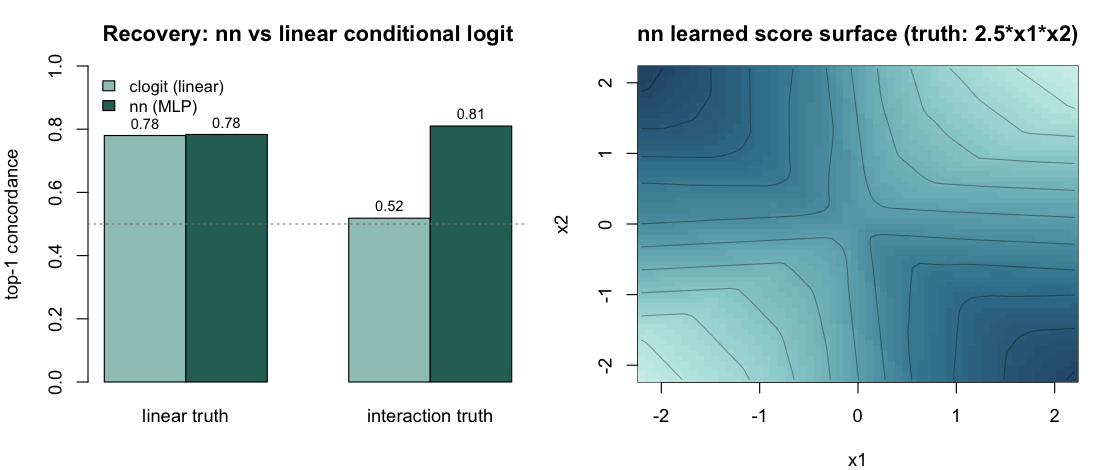
\includegraphics[width=0.9\textwidth]{figs/exp6-nn.png}
\caption{E6 neural backend. Left: in-sample top-1 concordance of \code{nn}
versus \code{clogit} under the linear and interaction truths. Right: the
learned score surface over $(x_1, x_2)$, reproducing the saddle of the
$2.5\,x_1 x_2$ interaction.}
\label{fig:val-e6}
\end{figure}

\subsection{E7: Additive-spline backend recovery, mini-batch invariance, and scaling}
\label{sec:val-e7}

The additive-spline architecture of Section~\ref{sec:framework-nn-additive}
--- per-covariate B-spline expansions trained by stochastic gradient on the
exact case-control partial likelihood, the STREAM construction of
\citet{filippimazzola2024} --- is checked on three properties: recovery of
additive effect shapes, invariance to mini-batching, and scaling against the
in-memory \code{gam} backend. The data-generating intensity is additive,
$\eta = \sin(2x_1) + 0.8\,x_2 + 0 \cdot x_3$, combining a nonlinear, a linear,
and a null effect, with one event and one sampled control per stratum.

Over ten Monte-Carlo replicates of $2{,}000$ strata
(Table~\ref{tab:val-e7-recovery}), the fitted curves recover the nonlinear and
linear effects (correlation $0.97$--$0.99$ with the centered truth) while the
null effect stays near-flat (amplitude $\approx 0.17$ against a unit-scale
signal). The fit is essentially identical under full-batch and mini-batch
training (\code{batch\_strata} of 256 and 64), and the additive-spline backend
improves top-1 concordance over the linear conditional logit ($0.74$ versus
$0.68$) by capturing the $\sin$ curvature the linear fit cannot represent
(Figure~\ref{fig:val-e7}, left).

\begin{table}[ht]
\centering\small
\begin{tabular}{lrrrr}
\toprule
Training & cor$(\hat f_1,\sin)$ & cor$(\hat f_2,\mathrm{lin})$ & null $\max|\hat f_3|$ & concordance \\
\midrule
full-batch & 0.974 & 0.994 & 0.176 & 0.739 \\
mini-batch (256) & 0.978 & 0.997 & 0.153 & 0.740 \\
mini-batch (64)  & 0.976 & 0.996 & 0.186 & 0.740 \\
linear \code{clogit} & --- & --- & --- & 0.676 \\
\bottomrule
\end{tabular}
\caption{E7 recovery and mini-batch invariance, averaged over ten replicates.}
\label{tab:val-e7-recovery}
\end{table}

On scaling (single fit at $2$k--$64$k strata), the additive-spline SGD is
faster and lighter than the \code{gam} fit on identical data, the gap widening
with size: at $64{,}000$ strata it runs in $8.1$\,s and $342$\,MB against the
\code{gam} backend's $12.7$\,s and $402$\,MB (Figure~\ref{fig:val-e7}, right).
This is the regime STREAM targets, here measured at modest scale on commodity
hardware; absolute timings are machine-dependent and were corroborated on a
second host.

\begin{figure}[ht]
\centering
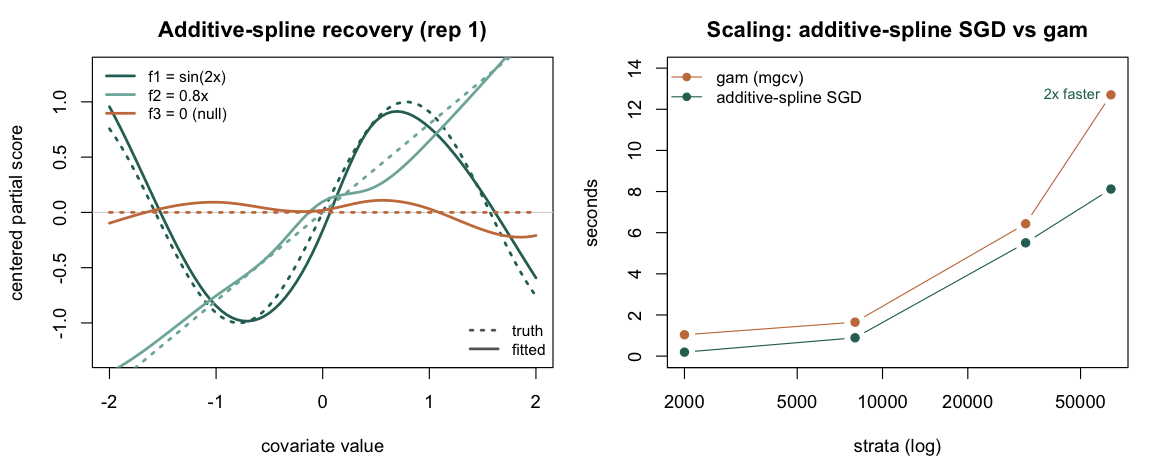
\includegraphics[width=\textwidth]{figs/exp7-additive.png}
\caption{E7 additive-spline backend. Left: fitted partial-effect curves
(solid) against the centered truths (dotted) for the nonlinear, linear, and
null covariates. Right: wall-clock scaling of additive-spline stochastic
gradient against the \code{gam} backend on the same case-control table.}
\label{fig:val-e7}
\end{figure}

Taken together, E1--E7 certify the simulator/likelihood consistency for
linear and smooth effects (E1, E2), the robustness of the naive
case-control estimator to actor-activity heterogeneity (E3), the relative
scaling and the honest failure boundaries of the two simulation kernels
(E4), the exact agreement of the simulator and post-hoc statistics engines
under correct history alignment (E5), and the correctness and
interaction-recovery behavior of the neural backend (E6), and the recovery, mini-batch invariance, and favorable scaling of the additive-spline backend against the in-memory smooth fit (E7). The two corrected
findings (E3 and E5) are reported in full because the test infrastructure
that produced the corrections --- the 48-file, $\sim$3{,}280-assertion suite
and the cross-implementation oracle --- is part of what \pkg{amore} offers.

\section{Empirical illustration}
\label{sec:illustration}

The preceding sections describe the components of \pkg{amore} in isolation.
This section ties them together into the workflow a practitioner actually
runs, on two of the nine bundled datasets (Section~\ref{sec:software-data}): a
small, homogeneous face-to-face stream (\texttt{classroom\_events}) and a
larger, heavy-tailed email network (\texttt{radoslaw\_email}). The first
reproduces the central methodological lesson of \citet{juozaitiene2024} ---
that the count family silently absorbs actor heterogeneity --- and shows how
a sender frailty term diagnoses it. The second illustrates the smooth
backend recovering non-monotone effect shapes. All numbers and figures
restated below are produced by the package's reproducible driver
(\texttt{paper/wiki/experiments/realdata.R}) and are reported, unchanged,
from the package's real-data analysis article; we do not re-estimate them
here.

Before either fit, it is worth recalling why these two streams stress the
machinery differently. The bundled event-rate trace
(Figure~\ref{fig:illustration-rate}) shows that the datasets are emphatically
non-stationary: the classroom stream has two sharp spikes (its two recorded
sessions) on an otherwise quiet baseline, whereas the manufacturing email
stream carries a visible weekly modulation over a roughly stationary base
rate. The per-actor degree distributions differ even more sharply ---
\texttt{classroom\_events} is bell-shaped on a tight log axis (a small
homogeneous group), while \texttt{radoslaw\_email} is heavy-tailed across
orders of magnitude, a small core driving most of the traffic. That
heterogeneity is precisely what the count family can mistake for dynamics.

\begin{figure}[t]
  \centering
  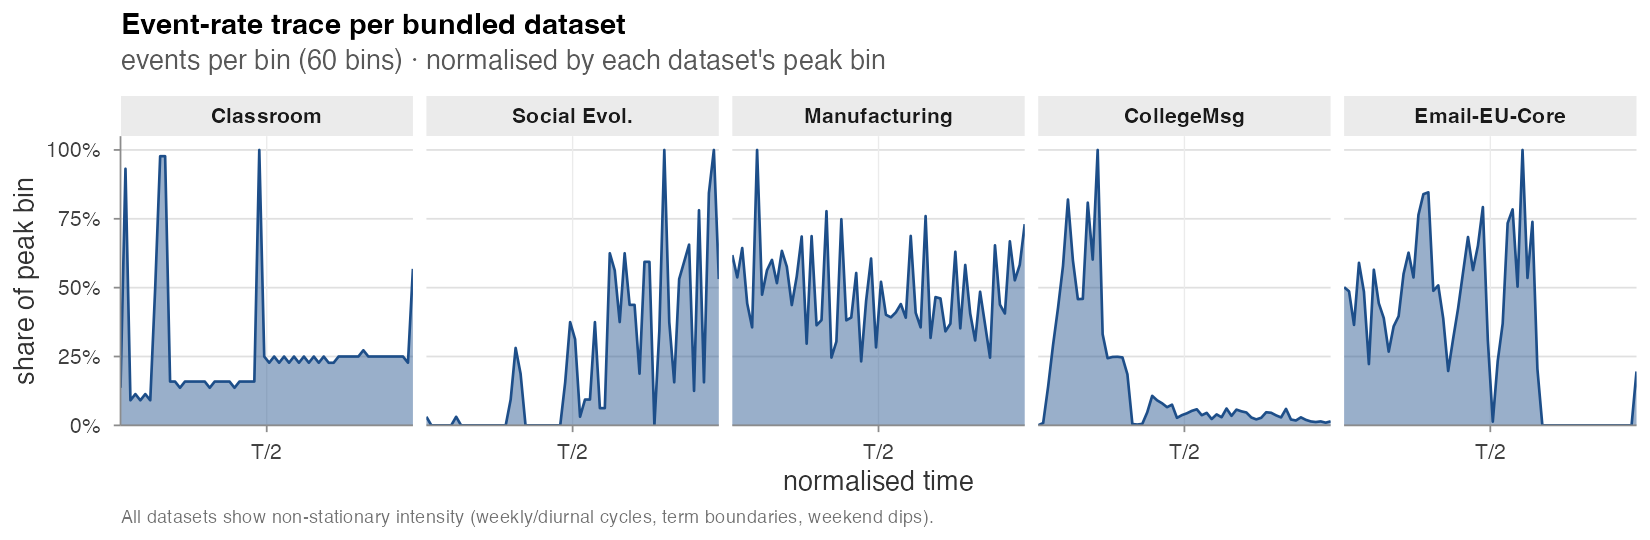
\includegraphics[width=0.95\textwidth]{figs/datasets-rate.png}
  \caption{Per-bin event-rate traces for the bundled datasets. The classroom
  stream (two session spikes) and the manufacturing email stream (weekly
  modulation on a stationary base) span the two regimes exercised in this
  section.}
  \label{fig:illustration-rate}
\end{figure}

\subsection{The common workflow}
\label{sec:illustration-workflow}

Every analysis in \pkg{amore} follows the same three steps: draw a
case--control sample of non-events, attach the endogenous statistics to the
resulting strata, and fit. The first two steps are backend-agnostic; only
the final \code{rem()} call (or, for the actor-heterogeneity diagnostic
below, \code{compare\_models()}) chooses an estimator. In code:

\begin{verbatim}
data(classroom_events)

cc   <- sample_non_events(classroom_events, n_controls = 3, seed = 11)
feat <- compute_endogenous_features(
  cc, stats = c("reciprocity_time_recent", "transitivity_time_recent"),
  history_log = classroom_events)

fit  <- rem(event ~ reciprocity_time_recent + transitivity_time_recent,
            data = feat, method = "clogit")
\end{verbatim}

\noindent The \code{sample\_non\_events()} call materialises, for each
observed event, a risk set of three sampled non-events; \code{compute\_%
endogenous\_features()} evaluates the requested statistics on the true
network history at each event time --- passing the original
stream as \code{history\_log} is essential here, so that only realised
events update the running network state while sampled controls read it
without writing to it (the alignment requirement established by experiment
E5 of Section~\ref{sec:validation}); and \code{rem(method =
"clogit")} maximises the risk-set softmax conditional-logistic partial
likelihood over the resulting strata. Swapping \code{method = "gam"}
substitutes the algebraically related degenerate case--control logistic
regression and unlocks \code{mgcv} smooth and time-varying terms;
\code{method = "nn"} substitutes the pure-R neural backend, which maximises
the same partial likelihood as \code{clogit} but scores the full candidate
vector jointly. The data frame \code{feat} is reused verbatim across all
three.

\subsection{Classroom: sender frailty flips the AIC ranking}
\label{sec:illustration-classroom}

The classroom stream (691 events, 20 actors, recorded in minutes;
\citealp{McFarland2001}) is small enough to refit repeatedly, which makes it
the natural vehicle for the actor-heterogeneity lesson. We compare three
effect specifications --- a \emph{count} family, a \emph{continuous}
(time-since-last) family, and the \emph{interrupted} variant of
\citet{juozaitiene2024} --- using \code{compare\_models()}, which wraps the
sample/feature/fit pipeline and returns an AIC table:

\begin{verbatim}
specs <- list(
  count       = c("reciprocity_count", "transitivity_count"),
  continuous  = c("reciprocity_time_recent", "transitivity_time_recent"),
  interrupted = c("reciprocity_time_recent_interrupted",
                  "transitivity_time_recent_interrupted"))

compare_models(classroom_events, specs, n_controls = 3, seed = 11)
#>         model n_terms n_obs  log_lik      AIC delta_AIC
#> 1       count       2   691 -5248.2 11880.5     0.0
#> 2  continuous       2   691 -5368.1 12120.2   239.7
#> 3 interrupted       2   691 -5449.8 12283.6   403.1
\end{verbatim}

Read naively, the count specification wins decisively, by 240 AIC points
over the continuous family. This is the trap: on a dataset with
heterogeneous senders the \texttt{*\_count} statistics absorb activity
differences directly, so they fit better for a reason that has nothing to do
with the timing dynamics the analyst cares about. The diagnostic is to add a
Gamma sender frailty (a \code{survival::frailty()} random effect on the
sender) and refit:

\begin{verbatim}
compare_models(classroom_events, specs, n_controls = 3, seed = 11,
               random_effects = "sender")
#>         model n_terms n_obs  log_lik      AIC delta_AIC
#> 1  continuous       2   691 -5177.7 11776.8     0.0
#> 2  interrupted       2   691 -5269.4 11960.5   183.7
#> 3       count       2   691      NA      NA     NA
\end{verbatim}

Two things happen, both shown in Figure~\ref{fig:realdata-classroom-flip}.
First, the count specification no longer fits at all: once the random effect
absorbs the activity differences, the inner Newton--Raphson update of the
frailty Cox fit fails to converge, and its AIC is undefined. Second, the
ranking among the remaining specifications flips --- continuous now overtakes
interrupted by 184 AIC points, matching Table~3 of \citet{juozaitiene2024}.
The lesson generalises: on heavy-tailed streams the naive AIC ranking
reflects who is active, not how the network evolves, and an actor-%
heterogeneity correction is the way to tell the two apart.

\begin{figure}[t]
  \centering
  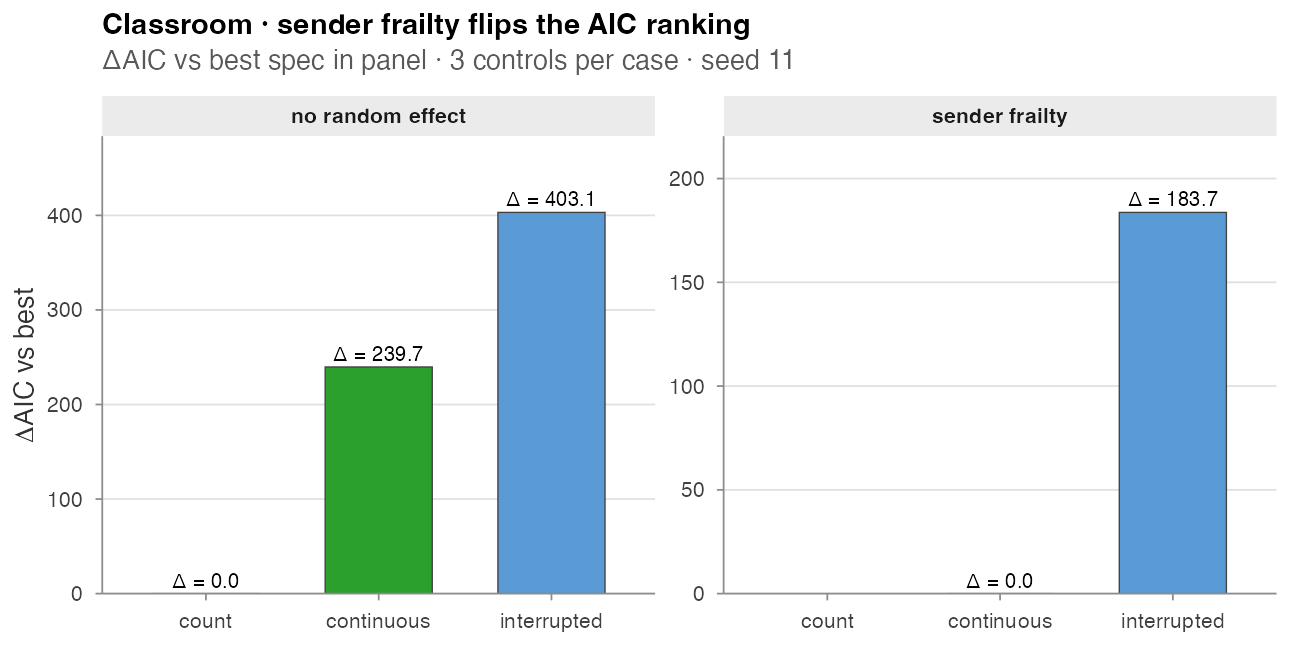
\includegraphics[width=0.9\textwidth]{figs/realdata-classroom-flip.png}
  \caption{Classroom AIC comparison without (left) and with (right) a Gamma
  sender frailty. Without the correction the count family leads by 240 AIC
  points; with it the count specification fails to converge and continuous
  overtakes interrupted by 184 points, reproducing Table~3 of
  \citet{juozaitiene2024}.}
  \label{fig:realdata-classroom-flip}
\end{figure}

\subsection{Manufacturing email: smooth effect curves}
\label{sec:illustration-smooth}

The same workflow, with \code{method = "gam"} in place of \code{clogit},
recovers the \emph{shape} of an endogenous effect rather than a single
coefficient. We use the first 30 days of the manufacturing email stream
(\texttt{radoslaw\_email}; \citealp{michalski2014}), restricted to
non-self-loops, and request smooth (penalised-spline) terms on four
statistics --- the continuous reciprocity and transitivity effects and their
interrupted variants:

\begin{verbatim}
data(radoslaw_email)
re30 <- radoslaw_email[radoslaw_email$time < 30, ]
re30 <- re30[re30$sender != re30$receiver, ]

stat_names <- c("reciprocity_time_recent",
                "transitivity_time_recent",
                "reciprocity_time_recent_interrupted",
                "transitivity_time_recent_interrupted")

cc   <- sample_non_events(re30, n_controls = 3, seed = 11)
feat <- compute_endogenous_features(cc, stats = stat_names)
\end{verbatim}

\noindent Fitting penalised splines on each statistic (via the smooth
backend, equivalently a stratified \code{pspline} Cox fit) yields the four
partial-effect curves in Figure~\ref{fig:realdata-manufacturing-smooth}. The
panels are not redundant. The continuous variants (top row) show the
canonical \emph{boost-then-decay} shape: a recent event briefly raises the
hazard, after which the contribution falls off and turns negative. The
interrupted variants (bottom row) start near zero, dip to a pronounced
minimum, and partially recover --- the cycle-closure-reset behaviour the
interrupted family is built to expose. Once the closing event fires, the
statistic snaps to a fresh state, and the partial effect on subsequent
events reflects that reset. A purely linear specification would collapse
each of these curves to a single slope and miss the non-monotonicity
entirely; this is the regime in which the smooth backend earns its place.

\begin{figure}[t]
  \centering
  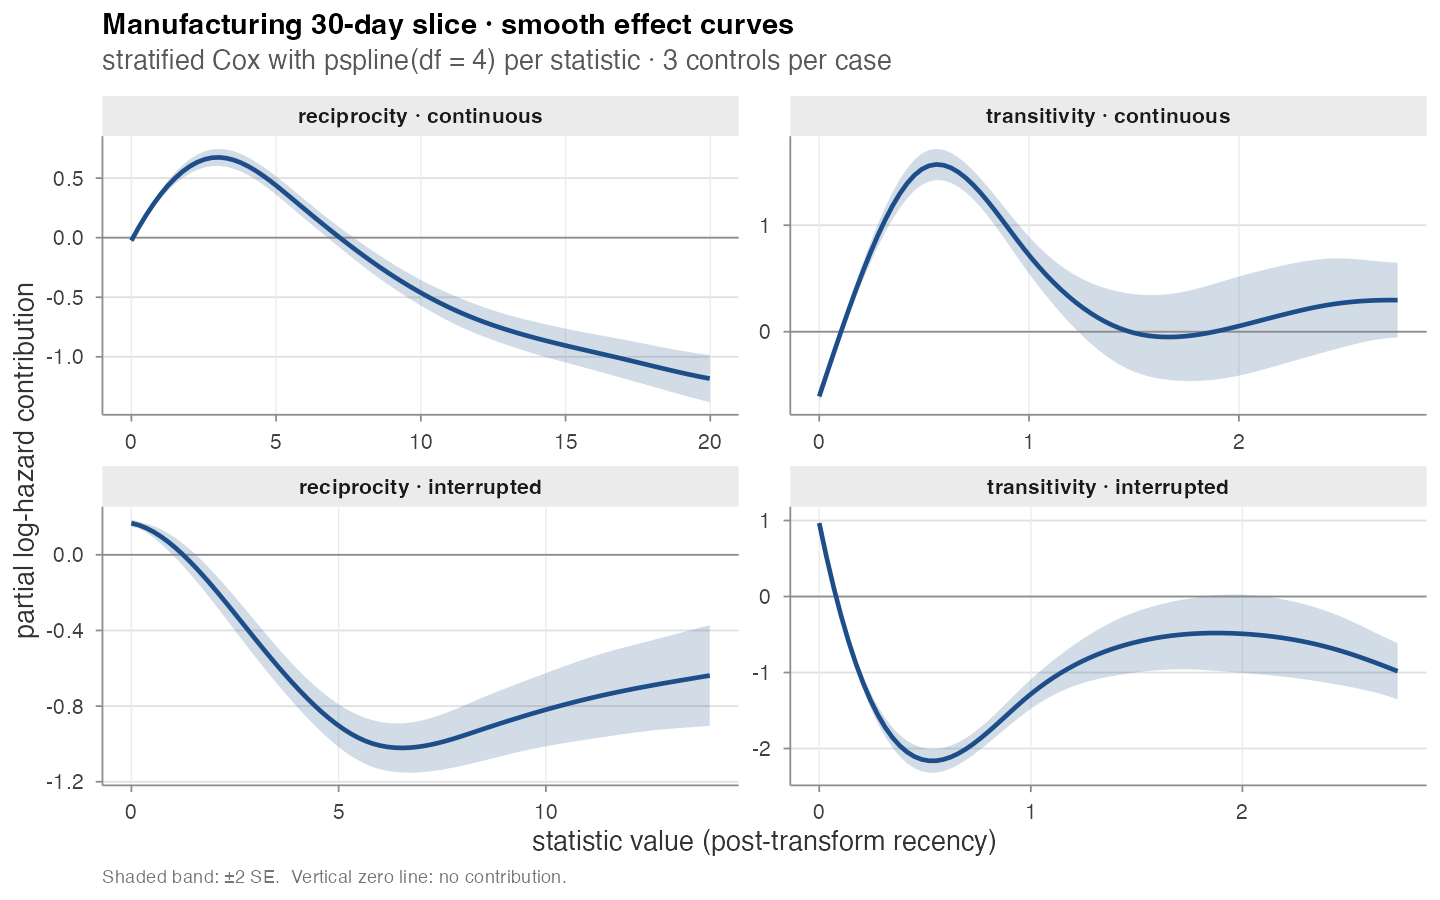
\includegraphics[width=0.95\textwidth]{figs/realdata-manufacturing-smooth.png}
  \caption{Penalised-spline partial-effect curves on the first 30 days of the
  manufacturing email stream. Continuous reciprocity and transitivity (top)
  show boost-then-decay; their interrupted variants (bottom) show the
  cycle-closure-reset dip and partial recovery.}
  \label{fig:realdata-manufacturing-smooth}
\end{figure}

\subsection{What the illustration does and does not show}
\label{sec:illustration-scope}

Taken together, the two analyses exercise the full front end on real data:
case--control sampling, the endogenous-statistics engine, the linear
conditional-logit fit, the smooth backend, and an actor-heterogeneity
diagnostic, all sharing one data structure. Two honest caveats apply. First,
the worked examples here use the \code{clogit} and \code{gam} backends; the
neural \code{nn} backend is demonstrated separately on a controlled planted-%
interaction design (Section~\ref{sec:validation}), where ground truth is
available, rather than on these streams, because its concordance figures are
in-sample and it carries no uncertainty quantification. Second, the
goodness-of-fit family (Section~\ref{sec:software-gof}) applies to the linear
case--control fit only; it is not exercised on the smooth manufacturing fit.
Within those bounds, the illustration demonstrates that the consolidated
workflow reproduces a published methodological finding
(\citealp{juozaitiene2024}, Table~3) end to end, from \code{data()} to AIC
table, in a single package.

\section{Discussion}
\label{sec:discussion}

\subsection{What the package gives a practitioner}
\label{sec:disc-summary}

\pkg{amore} closes the full relational-event analysis loop inside a single
\proglang{R} package. From a raw event stream a practitioner can: canonicalize
it into an \code{amore\_event\_log}; draw matched non-events under several risk-set
scopes; compute a catalogue of 74 numeric endogenous statistics spanning the
timing and closure variant axes; fit the resulting case-control table
through one \code{rem()} front-end; and, for the linear fit, run the
martingale-residual goodness-of-fit family of \citet{boschi2025gof}. The same
package also simulates: an exact Gillespie scheme and an approximate
$\tau$-leap scheme share one endogenous-state machine, and the simulator emits a
first-class case-control table that feeds \code{rem()} directly.

The expository spine is one likelihood with three predictors. The \code{clogit}
and \code{nn} backends maximize the \emph{same} risk-set softmax
conditional-logistic partial likelihood --- a linear predictor in the first
case, a hand-derived multilayer perceptron in the second --- while the
\code{gam} backend fits the algebraically related degenerate (case-1-control)
binomial logistic regression of \citet{boschi2025rhem} via \pkg{mgcv}, giving
access to smooth, time-varying, and random-effect terms. The validation battery
(Section~\ref{sec:validation}) supports the implementation: linear effects are
recovered with bias $\le 0.006$ for $|\beta| \le 0.4$ and Wald coverage between
0.90 and 1.00 (E1); a non-linear smooth is recovered with RMSE 0.075 and
correlation 0.998 (E2); the simulator and the post-hoc feature engine agree to
$4.3\times 10^{-14}$ under history-log alignment (E5); and the neural gradients
match numerical differentiation to $1.4\times 10^{-10}$ (E6). The contribution
is the integrated, reproducible artifact and its unifying frame --- not new
statistical theory.

\subsection{Limitations}
\label{sec:disc-limitations}

We state the boundaries of the package plainly, because several of them
constrain how the tool should be used.

\paragraph{Goodness of fit is linear-only.} The four \code{gof\_*} functions and
\code{martingale\_residuals()} operate on the linear case-control fit and hard-reject
anything else; there is no goodness-of-fit machinery for the smooth (\code{gam})
or neural (\code{nn}) backends. The recentering step that aligns the residual
process is a heuristic, and we have not conducted a calibration or power study of
the tests themselves.

\paragraph{The neural backend is deliberately minimal.} The \code{nn} backend is
pure R and GPU-free, training full-batch by default with optional
mini-batching. Its analytic gradients are verified against
numerical differentiation, but the design carries real costs: it returns no
coefficients, standard errors, or any other uncertainty quantification
(\code{coef()} is \code{NULL}); it rejects factor covariates and accepts numeric
inputs only; and the pure-R training loop sets a practical scalability ceiling below a
compiled engine --- mitigated, but not removed, by the mini-batch option. The interaction-recovery
advantage reported in E6 (concordance 0.81 for \code{nn} versus 0.52 for
\code{clogit} on a planted $x_1 x_2$ truth, against ties of 0.78/0.78 on a linear
truth) is an \emph{in-sample} metric on a single fixture; it is evidence that the
joint MLP can represent structure the additive backends cannot, not a
generalization guarantee. We frame this backend strictly as an accessibility and
engineering contribution, with no priority claim: STREAM
\citep{filippimazzola2024} already fits flexible additive effects on the same
case-control objective at far larger scale, and neural temporal-point-process
models \citep{du2016,mei2017} long predate this package.

\paragraph{The simulator has small-network failure modes.} The scaling study (E4)
shows $\tau$-leap is 22--42$\times$ faster than Gillespie at 60 actors and up to
roughly $100\times$ at 100 actors. But both schemes break down at \emph{small}
actor counts under a strongly self-exciting process, for opposite reasons:
Gillespie's per-dyad softmax underflows (``too few positive probabilities'') and
$\tau$-leap's intensities blow up into a memory overflow. A practitioner
simulating small, strongly self-exciting networks should expect to tune the time
step, reduce the effect strength, or accept that some configurations are not
reachable with either engine.

\paragraph{Naming and release status.} The package name shares letters with the
archived CRAN package \code{AMORE} (a neural-network toolbox), which must be
resolved before a CRAN submission. As of this writing the headline backends and
the full statistics engine are present in the source tree; a clean CRAN
re-release exposing them through the installed binary is a prerequisite for the
package to deliver its advertised interface to a user running
\code{install.packages("amore")}.

\paragraph{Hyper-event support is rem-ready but undemonstrated.} The relational
hyper-event (RHEM) feature path --- hyperedge simulation and hyperedge feature
computation --- exists and produces case-control tables of the shape
\code{rem()} consumes. We have not yet shipped a vignette carrying a single
end-to-end \code{rem()} fit on hyper-event data, so RHEM should be read as a
designed-and-wired capability rather than a demonstrated one.

\subsection{Future work}
\label{sec:disc-future}

Several extensions follow directly from the limitations above and would
strengthen the package without altering its frame.

\begin{itemize}
  \item A compiled, minibatched neural engine (e.g.\ a \pkg{torch} backend)
        would lift the pure-R scalability ceiling and make larger event logs
        tractable for the \code{nn} backend.
  \item Factor support via embeddings would let the neural backend consume the
        categorical actor and dyad attributes it currently rejects.
  \item Uncertainty quantification for the neural fit --- bootstrap, or an
        approximate posterior --- would turn its point predictions into
        inferential statements comparable to the linear backend's Wald intervals.
  \item Extending the goodness-of-fit family beyond the linear case-control fit,
        to the smooth and neural backends, would close the most conspicuous gap
        in the current toolchain.
  \item Penalization and basis selection for the additive-spline
        architecture (currently unpenalized, with fixed degrees of freedom per
        covariate, as in \citealp{filippimazzola2024}), and resampling-based
        uncertainty bands for its fitted curves.
  \item A worked end-to-end \code{rem()} fit on hyper-event data would convert the
        RHEM path from a wired capability into a demonstrated one.
\end{itemize}

In its present form \pkg{amore} consolidates a methodology that previously lived
as scattered scripts and a separate simulation tool into one coherent, tested,
documented package, organized around a single unifying view of the
relational-event likelihood. That consolidation, and the reproducible evidence
that the pieces work together correctly, is the contribution we claim.


\bibliographystyle{abbrvnat}
\bibliography{references}

\end{document}
